\documentclass[11pt,a4paper]{article}

\usepackage{gastex}
\usepackage{etoolbox}
% \newcommand{\showLoesung}{2} %<---als Schalter
%\newcommand{\showInhalt}{1} %<---als Schalter

\usepackage{alltt,moreverb,amsmath,enumerate}
\usepackage[normalem]{ulem}
\usepackage[T1]{fontenc}
\usepackage{ae,aecompl} %helvet,mathptm
%\usepackage[left=15mm,right=15mm,top=20mm,bottom=20mm]{geometry}
\usepackage[margin=.5in]{geometry}
%\usepackage[latin1]{inputenc} % f�r Linux
\usepackage[utf8]{inputenc} % Umlaute etc. direkt schreiben (unter Windows)
\usepackage[german]{babel}
\usepackage[url]{oth-logoPNG}
%\usepackage{i2sym,i2ams}

\usepackage{tikz}
\usetikzlibrary{arrows,shapes,trees,positioning,automata,decorations.pathreplacing,decorations.pathmorphing}
\usepackage{tkz-graph}
\usepackage{color}

\usepackage{longtable}
\usepackage{tabularx}

%\usepackage{epic}
%\usepackage{eepic}
\usepackage{comment,ifthen}
\usepackage{../include/todo}

\usepackage[T1]{fontenc}
\usepackage{textcomp}

\usepackage{listings}                   % Listings in Core-Erlang und Maude
\usepackage{lstmisc}

\usepackage{epic}                       % Bildbefehle (picture)
%\usepackage{eepic}                      % erweiterte Bildbefehle

\usepackage{bbm}                        % Mengensymbole (N,C,R,B)
\usepackage{latexsym}                   % zusaetzliche Mathesymbole
\usepackage{amsmath}                    % Mathepaket von der AMS
\usepackage{amstext}
\usepackage{amsfonts}
\usepackage{stmaryrd}                   % zusaetzliche Mathesymbole
\usepackage{mathtools}
\usepackage{amsthm}
\usepackage{cancel}

\usepackage{hyperref}
\usepackage{url}                        % Zum Setzen von URLs in typewriter-face

\pagestyle{empty}

\let\epsilon=\varepsilon
\let\phi=\varphi

\frenchspacing

\setlength{\parindent}{0pt}
\setlength{\textwidth}{18.6cm}
\setlength{\textheight}{26.5cm}
\setlength{\hfuzz}{1mm}

%%% Read dates of assignments from file
\usepackage{xparse}
\ExplSyntaxOn
\ior_new:N \g_hringriin_file_stream

\NewDocumentCommand{\ReadFile}{mm}
 {
  \hringriin_read_file:nn { #1 } { #2 }
  \cs_new:Npn #1 ##1
   {
    \str_if_eq:nnTF { ##1 } { * }
      { \seq_count:c { g_hringriin_file_ \cs_to_str:N #1 _seq } }
      { \seq_item:cn { g_hringriin_file_ \cs_to_str:N #1 _seq } { ##1 } }
   }
 }

\cs_new_protected:Nn \hringriin_read_file:nn
 {
  \ior_open:Nn \g_hringriin_file_stream { #2 }
  \seq_gclear_new:c { g_hringriin_file_ \cs_to_str:N #1 _seq }
  \ior_map_inline:Nn \g_hringriin_file_stream
   {
    \seq_gput_right:cx 
     { g_hringriin_file_ \cs_to_str:N #1 _seq }
     { \tl_trim_spaces:n { ##1 } }
   }
  \ior_close:N \g_hringriin_file_stream
 }

\ExplSyntaxOff

\ReadFile{\uebungsabgabe}{../skel/UEBUNGSABGABE.def}

%%% Read subject info from file
\newcommand{\dozent}[1]{\def\DOZENT{#1}}
\newcommand{\tutoren}[1]{\def\TUTOREN{#1}}
\newcommand{\vorlesung}[1]{\def\VORLESUNG{#1}}
\newcommand{\semester}[1]{\def\SEMESTER{#1}}

\InputIfFileExists{../skel/VORLESUNG.def}{\providecommand{\TUTOREN}{}}%
{\typeout{***********}
 \typeout{Warnung: Kein File vorhanden, das die Vorlesung spezifiziert!}
 \typeout{Spezifikation muss daher im Text des Blattes oder ueber die
          Tastatur erfolgen.}
 \typeout{***********}}

\def\Uebung#1#2#3{
  \othLehrstuhlLogo[\DOZENT]
  \begin{center}
	{~\\[-2em]\Large\bf \VORLESUNG}\\[0.5em]
    \LARGE --~Tutorium #1 (Übung #2)~--\\[4mm]
  \
  \normalsize
  \textbf{#3}
    \rule{\textwidth}{0.1pt}\\[1cm]
  \end{center}
}

\def\Hinweis#1{
	{~\\[-3em]\bf Hinweis: }
	\begin{minipage}[t]{16.5cm}
	#1
	\end{minipage}\\[1em]
    \rule{\textwidth}{0.1pt}
}

\def\Tipps#1{
	{~\\[-3em]\bf Tipps: }
	\begin{minipage}[t]{16.5cm}
	#1
	\end{minipage}\\[1em]
    \rule{\textwidth}{0.1pt}
}
  
\def\MyHeader{
  \othLehrstuhlLogo[Prof.~Dr.~rer.~nat.~Carsten~Kern]%[Carsten~Kern,~Stefan~Rieger]
}

\newcommand{\sem}[1]{[\![#1\,]\!]}

\def\aufgabe#1#2{\subsection*{Aufgabe #1 (#2)}\par}
\def\endaufgabe{}

\newenvironment{loesung}{\subsection*{L\"osungsvorschlag:}}{}
\newenvironment{hinweis}{}{}
\ifthenelse{\isundefined{\showLoesung}}{\excludecomment{loesung}}{\pagestyle{plain}\excludecomment{hinweis}}

\newenvironment{tipps}{}{}
\ifthenelse{\isundefined{\showTipps}}{\excludecomment{tipps}}{\excludecomment{hinweis}}

\newenvironment{inhalt}{\subsection*{Kommentar:}}{}
\ifthenelse{\isundefined{\showInhalt}}{\excludecomment{inhalt}}{}

\long\def\Exercise#1#2{\begin{exercise}{#1}#2\end{exercise}}

\def\underbar#1{%
  \setbox0=\hbox{#1}%
  \dimen0=\dp0\relax%
  \dp0=0pt%
  \setbox0=\hbox{\underline{\box0}}%
  \dp0=\dimen0\relax%
  \box0%
  }

\makeatletter
\def\@makeunderbar[#1]#2{\expandafter\def\csname#1\endcsname{\underbar{#2}}}
\def\makeunderbar{\@ifnextchar[{\@makeunderbar}{\@makeunderbar[]}}
\makeatother

\def\T{\mathrm{T}}
\def\P{\mathrm{P}}
\def\CT{\mathrm{CT}}
\def\COp{\mathrm{COp}}

\makeunderbar{Comp}
\makeunderbar{Ops}
\makeunderbar{trans}
\makeunderbar[strans]{s-trans}
\makeunderbar[ntrans]{n-trans}
\makeunderbar{fix}

\def\labelenumi{\alph{enumi})}
\let\<=\langle
\let\>=\rangle

\parindent=0pt
\parskip=1ex

\definecolor{javared}{rgb}{0.6,0,0} % for strings
\definecolor{javagreen}{rgb}{0.25,0.5,0.35} % comments
\definecolor{javapurple}{rgb}{0.5,0,0.35} % keywords
\definecolor{javadocblue}{rgb}{0.25,0.35,0.75} % javadoc
 
\lstset{language=C++,
basicstyle=\ttfamily\footnotesize,
keywordstyle=\color{javapurple}\bf,
stringstyle=\color{javared},
commentstyle=\color{javagreen}\it\bf,
morecomment=[s][\color{javadocblue}]{/**}{*/},
numbers=left,
numberstyle=\tiny\color{gray},
stepnumber=1,
numbersep=10pt,
tabsize=3,
showspaces=false,
showstringspaces=false}

\usepackage{enumitem}
\usepackage{algpseudocode}
\usepackage{caption}
\usepackage{subcaption}
\usepackage{placeins}
\usepackage{multicol}
\usepackage{tikz}
\usetikzlibrary{shapes}

\begin{document}
\thispagestyle{empty}

\Uebung{7}{8}{Simon Thelen}{25. November 2021}  % FIXME: Blattnummer, Datum, Zeit

%%%%%%%%%%%%%%%%%%%%%%%%%%%%%%%%%%%%%%%%%%%%%%%%%%%%%%%%%%%%%%%%%%%%%%

\ifcsdef{showLoesung}{
\textbf{Bitte beachten Sie:} Die Lösungen können trotz sorgfältiger Prüfung Fehler enthalten.
Bei Fragen oder Unklarheiten kontaktieren Sie bitte den Tutor oder Dozenten in Tutorien, Übungen oder nach Vorlesungen.
}{}

\begin{aufgabe}{1}{Suchbäume}
    \begin{enumerate}
        % \item Gegeben sei ein AVL-Baum mit $n$ Knoten.
        % Geben Sie geschlossene Formeln für die minimale und die maximale Höhe des Baumes an.
        \item Gegeben seinen $n$ ganze Zahlen.
        Es soll ein binär, verketter Suchbaum erzeugt werden, welcher genau die gegeben Zahlen enthält.
        Zeigen Sie, dass dies im Allgemeinen nicht schneller als in $\Omega\big(n \log(n)\big)$ möglich ist, wenn das Erstellen des Suchbaums mithilfe von Vergleichen erfolgt.
        \item Konvertieren Sie folgenden Suchbaum mittels Rechtsrotationen in einen entarteten Baum mit 1 als Wurzel.
        \begin{figure}[h!]
            \centering
            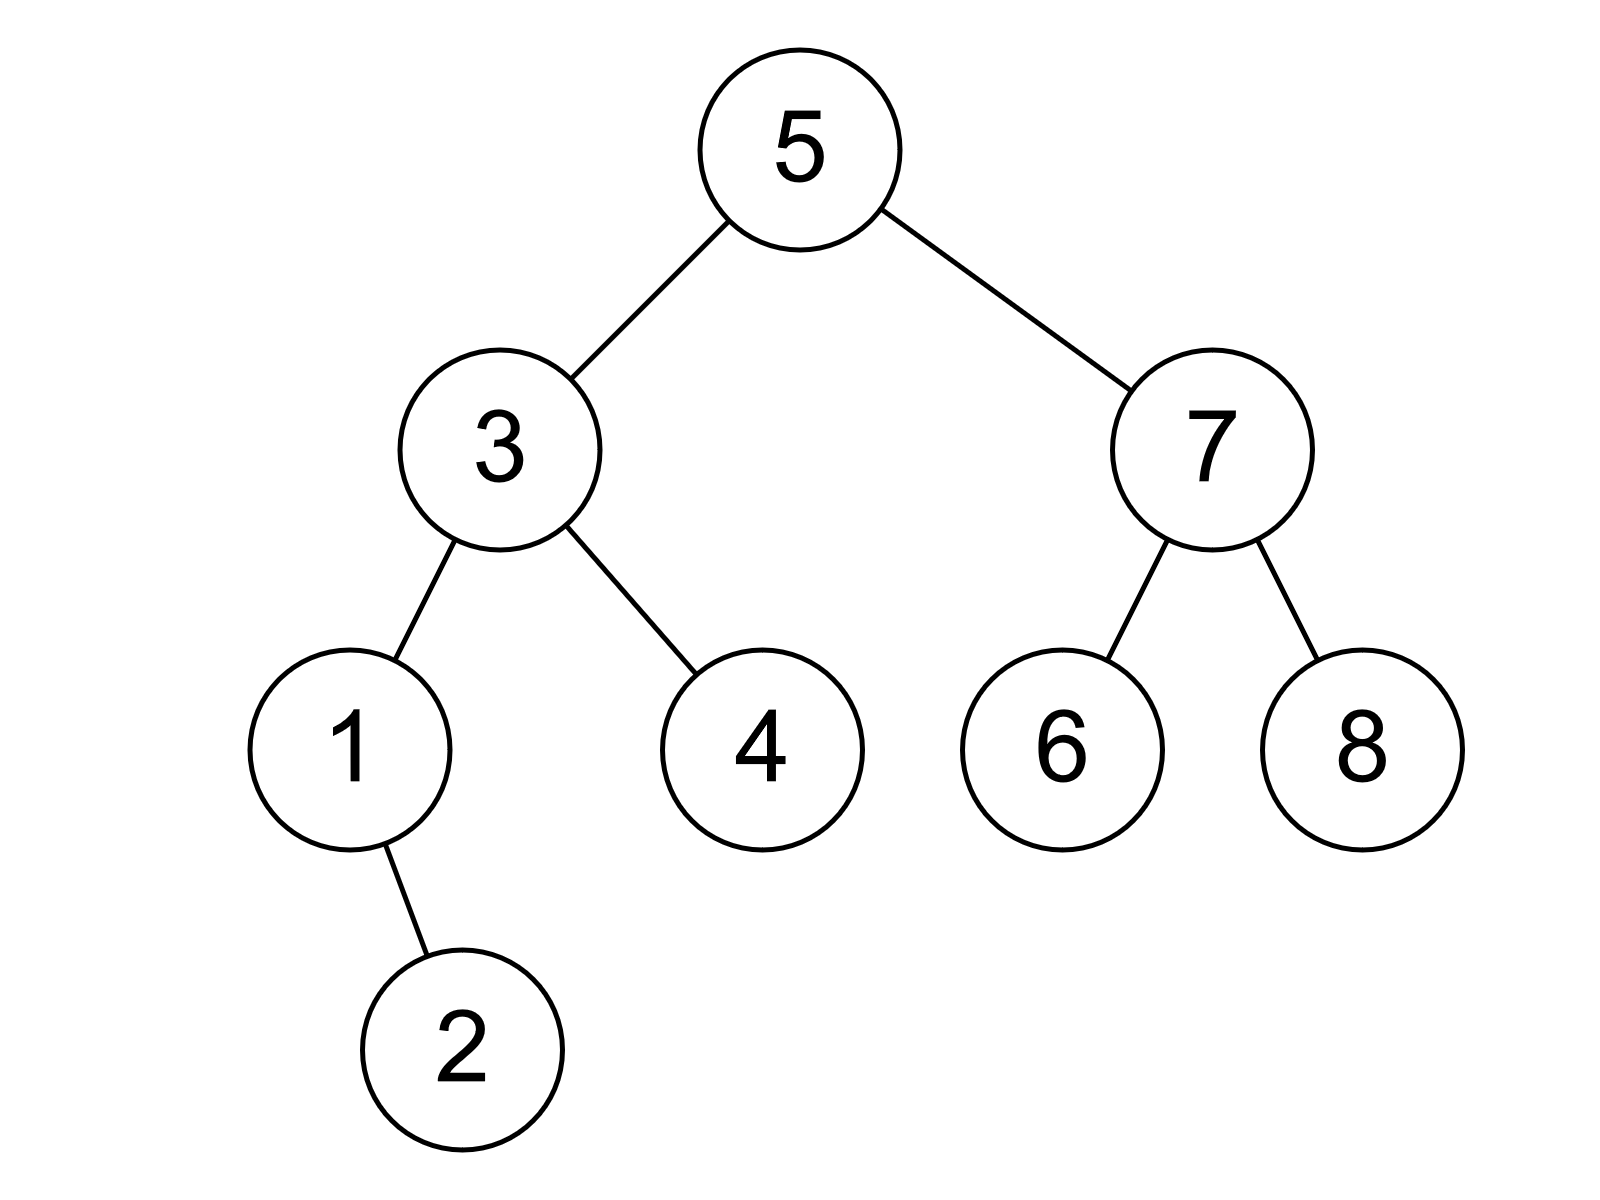
\includegraphics[width=0.22\textwidth]{img/1c}
        \end{figure}
        \FloatBarrier
        Wie viele Rechtsrotationen benötigen Sie?
        Zeigen Sie, dass Sie bei einem Suchbaum mit $n$ Knoten maximal $n - 1$ Rotationen benötigen, um den Baum in einen entarteten Baum zu konvertieren.
    \end{enumerate}
\end{aufgabe}

\begin{loesung}
    \begin{enumerate}
        \item
        \begin{proof}
            Beweis durch Widerspruch:
            Angenommen, es gäbe einen Algorithmus, der den Suchbaum mittels Vergleichen in $T(n) \not\in \Omega\big(n \log(n)\big)$ erzeugt. 
            Betrachte nun folgenden vergleichsbasierten Sortieralgorithmus:
            \begin{itemize}
                \item Erzeuge einen Suchbaum aus den $n$ zu sortierenden Werten.
                \item Durchlaufe den Suchbaum in Inorder-Reihenfolge und füge die Werte in ein Ausgabearray ein.
            \end{itemize}
            Die Werte eines Suchbaums, in Inorder-Reihenfolge durchlaufen, sind stets aufsteigend sortiert.
            Der Sortieralgorithmus ist also korrekt.
            Die Laufzeit des Algorithmus beträgt $O(n + T(n))$, was schneller ist als $\Omega\big(n \log(n)\big)$.
            Die untere Schranke für vergleichsbasiertes Sortieren ist jedoch $\Omega\big(n \log(n)\big)$.
            Daher kann der obige Algorithmus nicht schneller als $\Omega\big(n \log(n)\big)$ sein.
            Die ursprüngliche Annahme muss also falsch sein.
            Es gibt keinen vergleichsbasierten Algorithmus, der einen Suchbaum bestehend aus $n$ beliebigen Werten schenller als in $\Omega\big(n \log(n)\big)$ erzeugt.
        \end{proof}

        \item \ Es reichen 5 Rechtsrotationen:
        \begin{figure}[h!]
            \centering
            \begin{subfigure}[b]{0.23\textwidth}
                \centering
                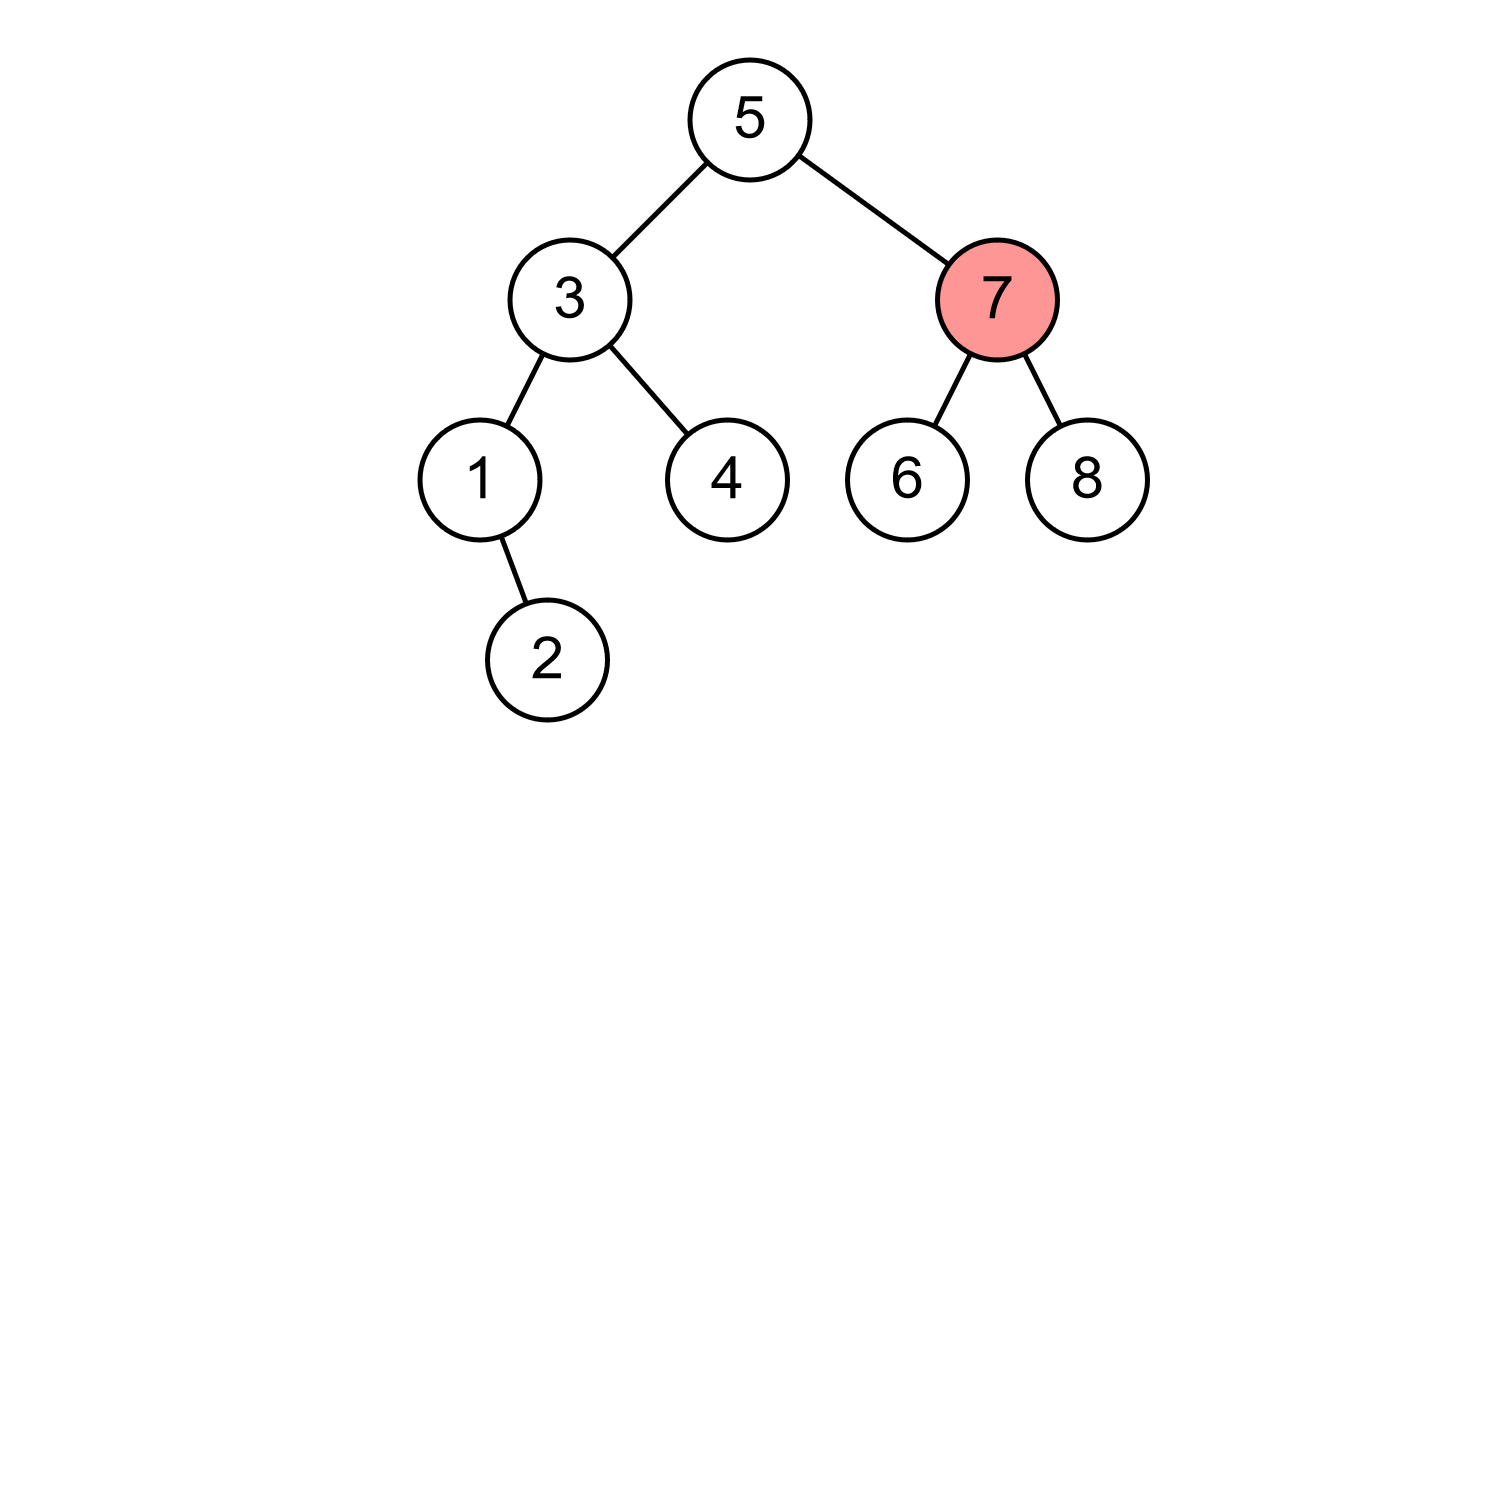
\includegraphics[width=\textwidth]{img/1b/2}
            \end{subfigure}
            \begin{subfigure}[b]{0.23\textwidth}
                \centering
                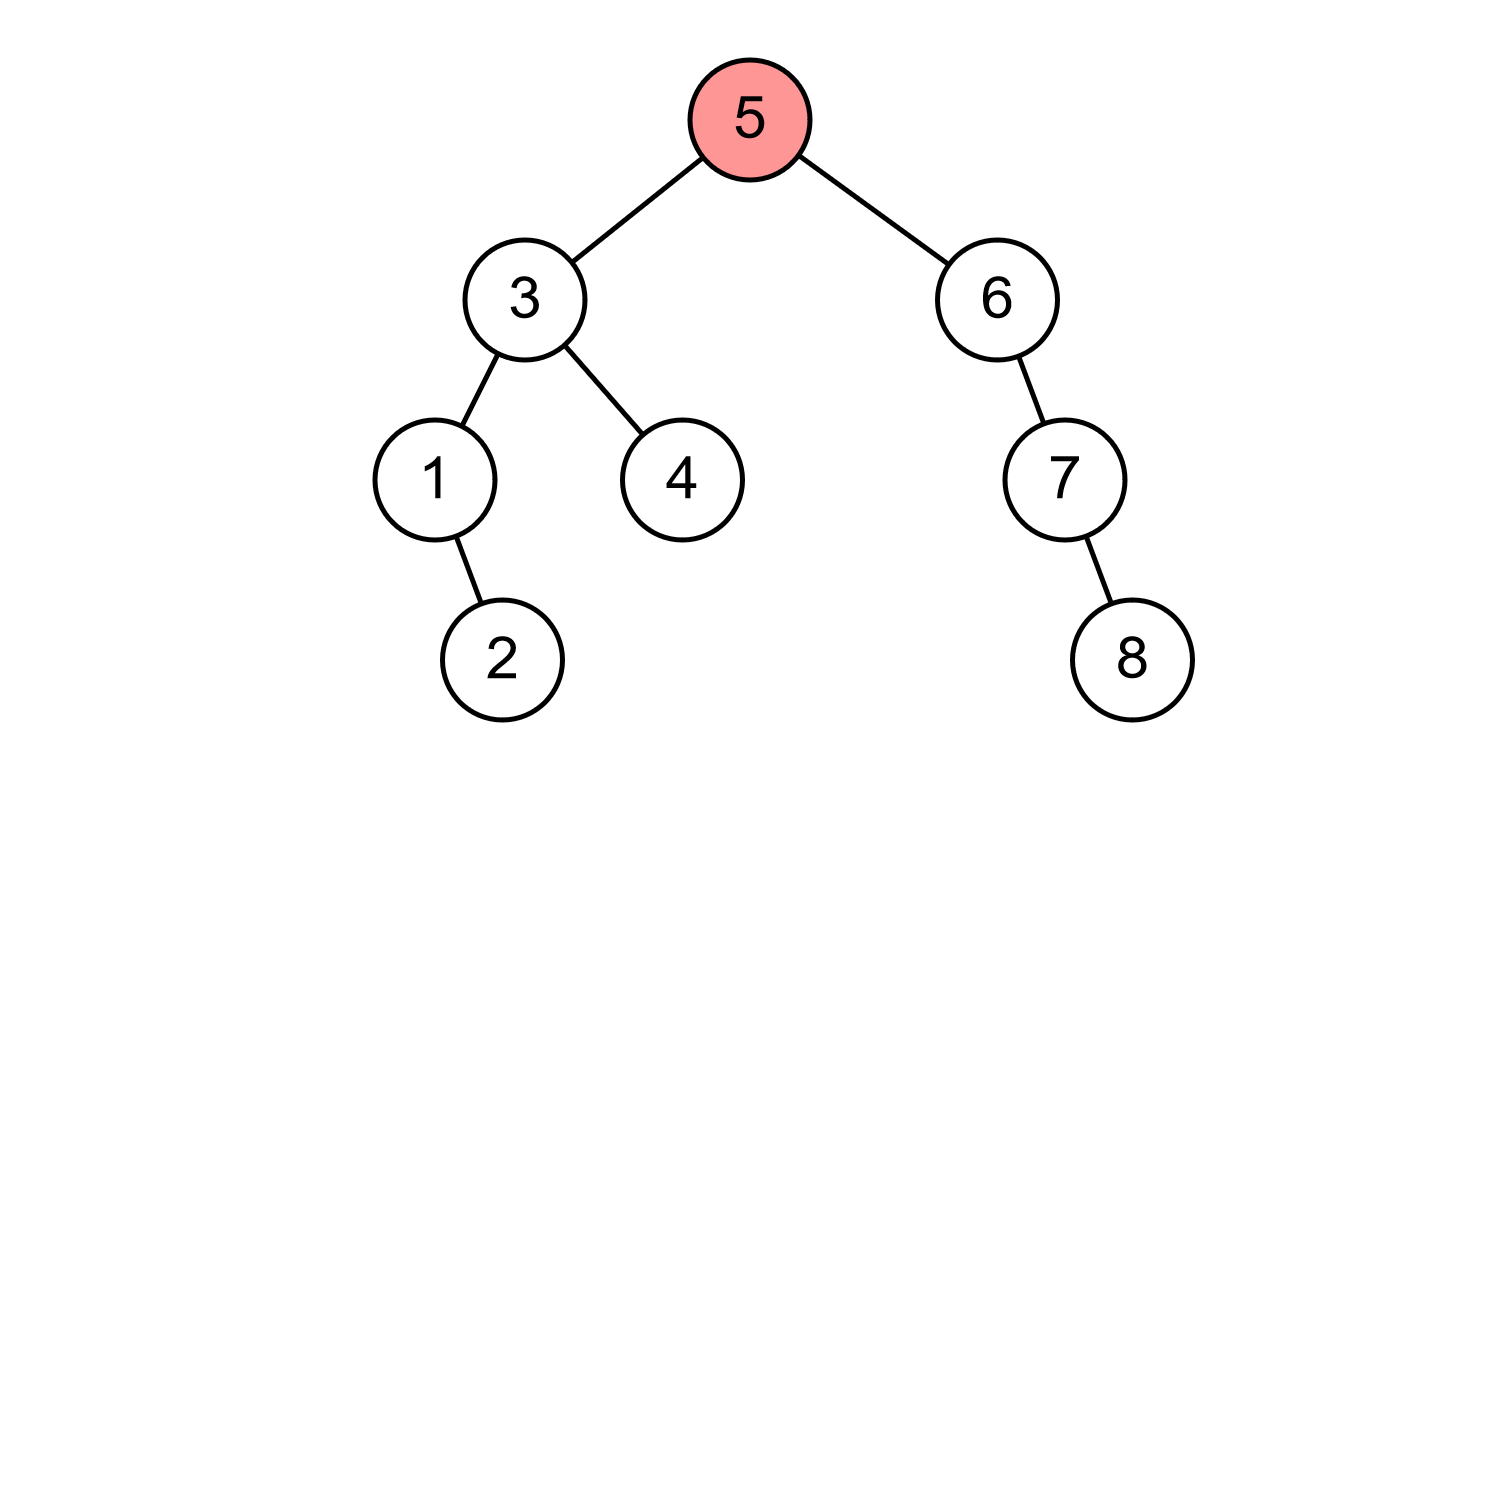
\includegraphics[width=\textwidth]{img/1b/3}
            \end{subfigure}
            \begin{subfigure}[b]{0.23\textwidth}
                \centering
                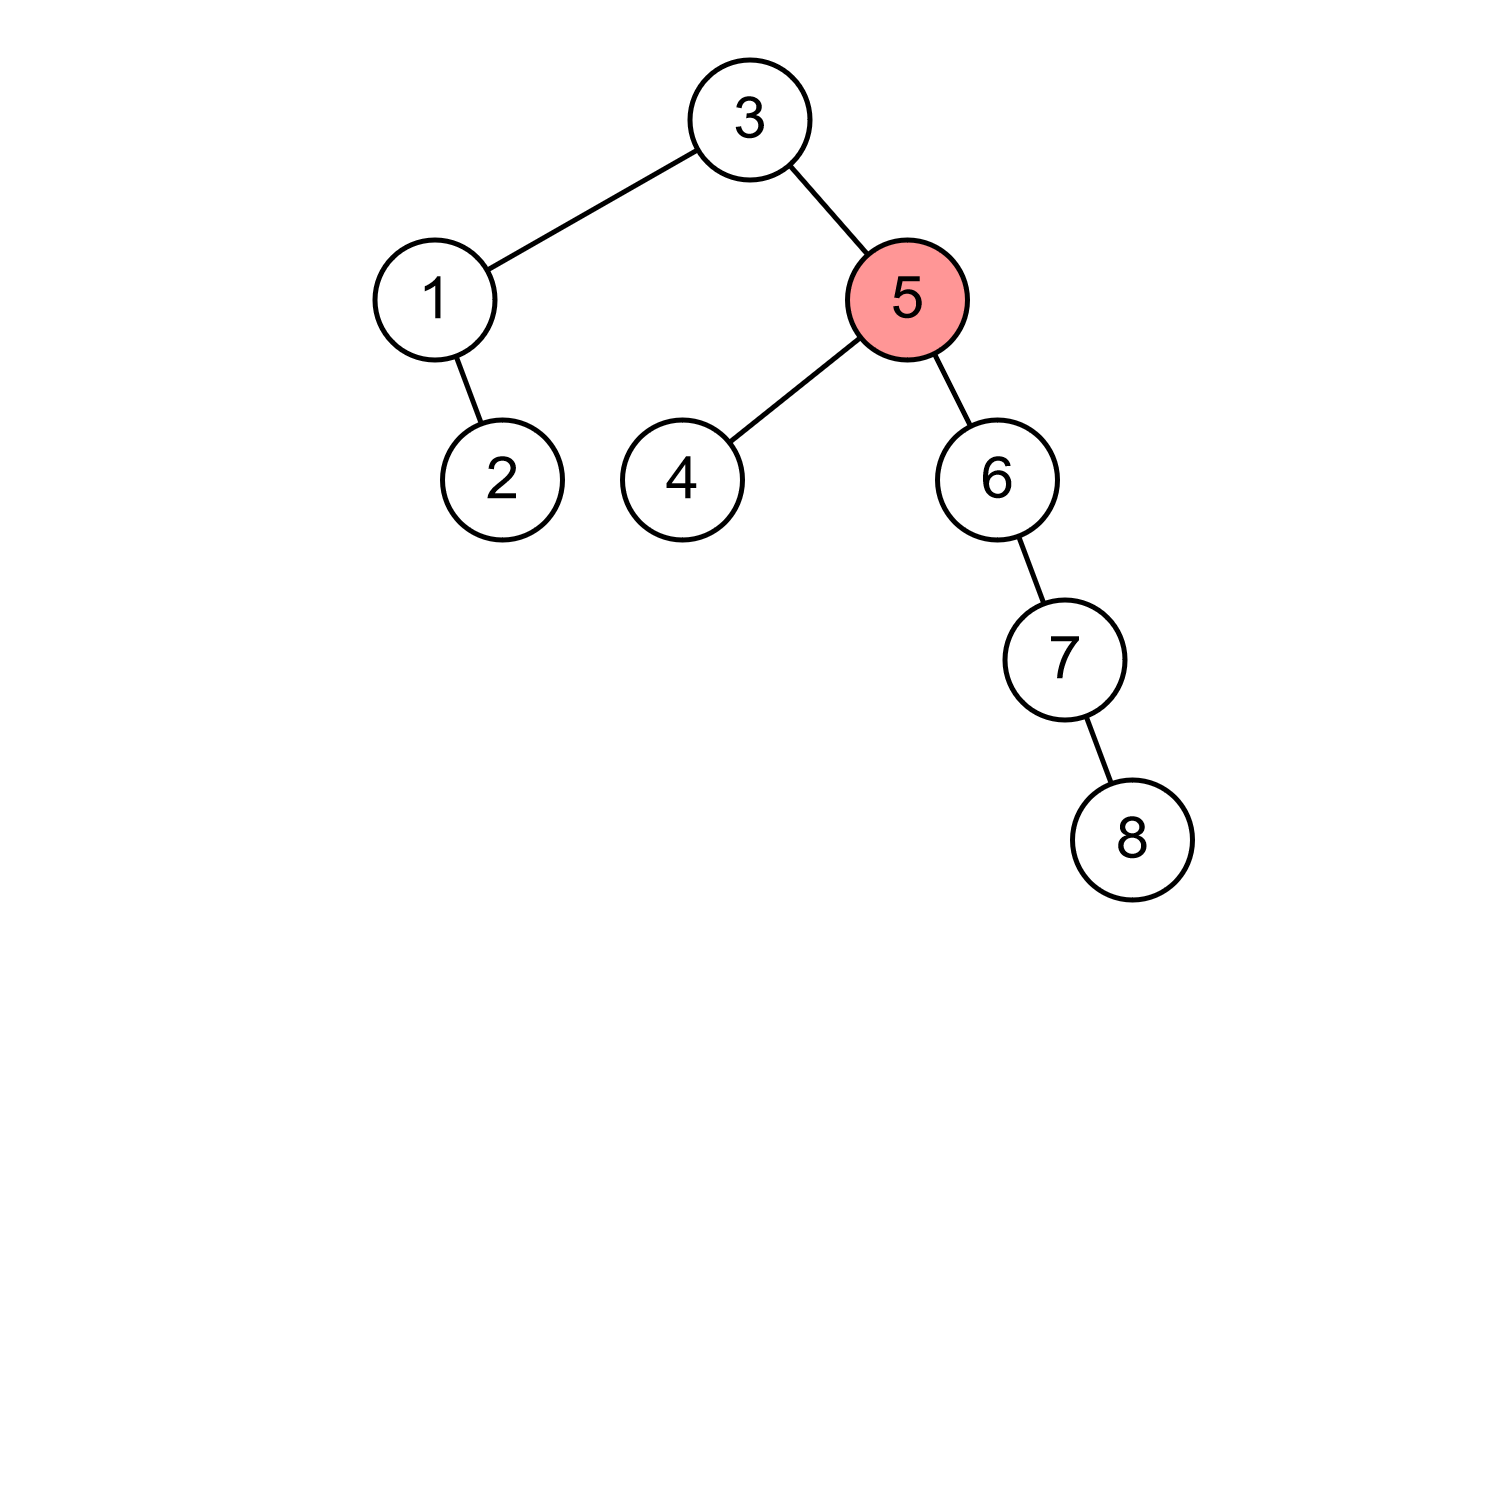
\includegraphics[width=\textwidth]{img/1b/4}
            \end{subfigure}
            \\
            \begin{subfigure}[b]{0.23\textwidth}
                \centering
                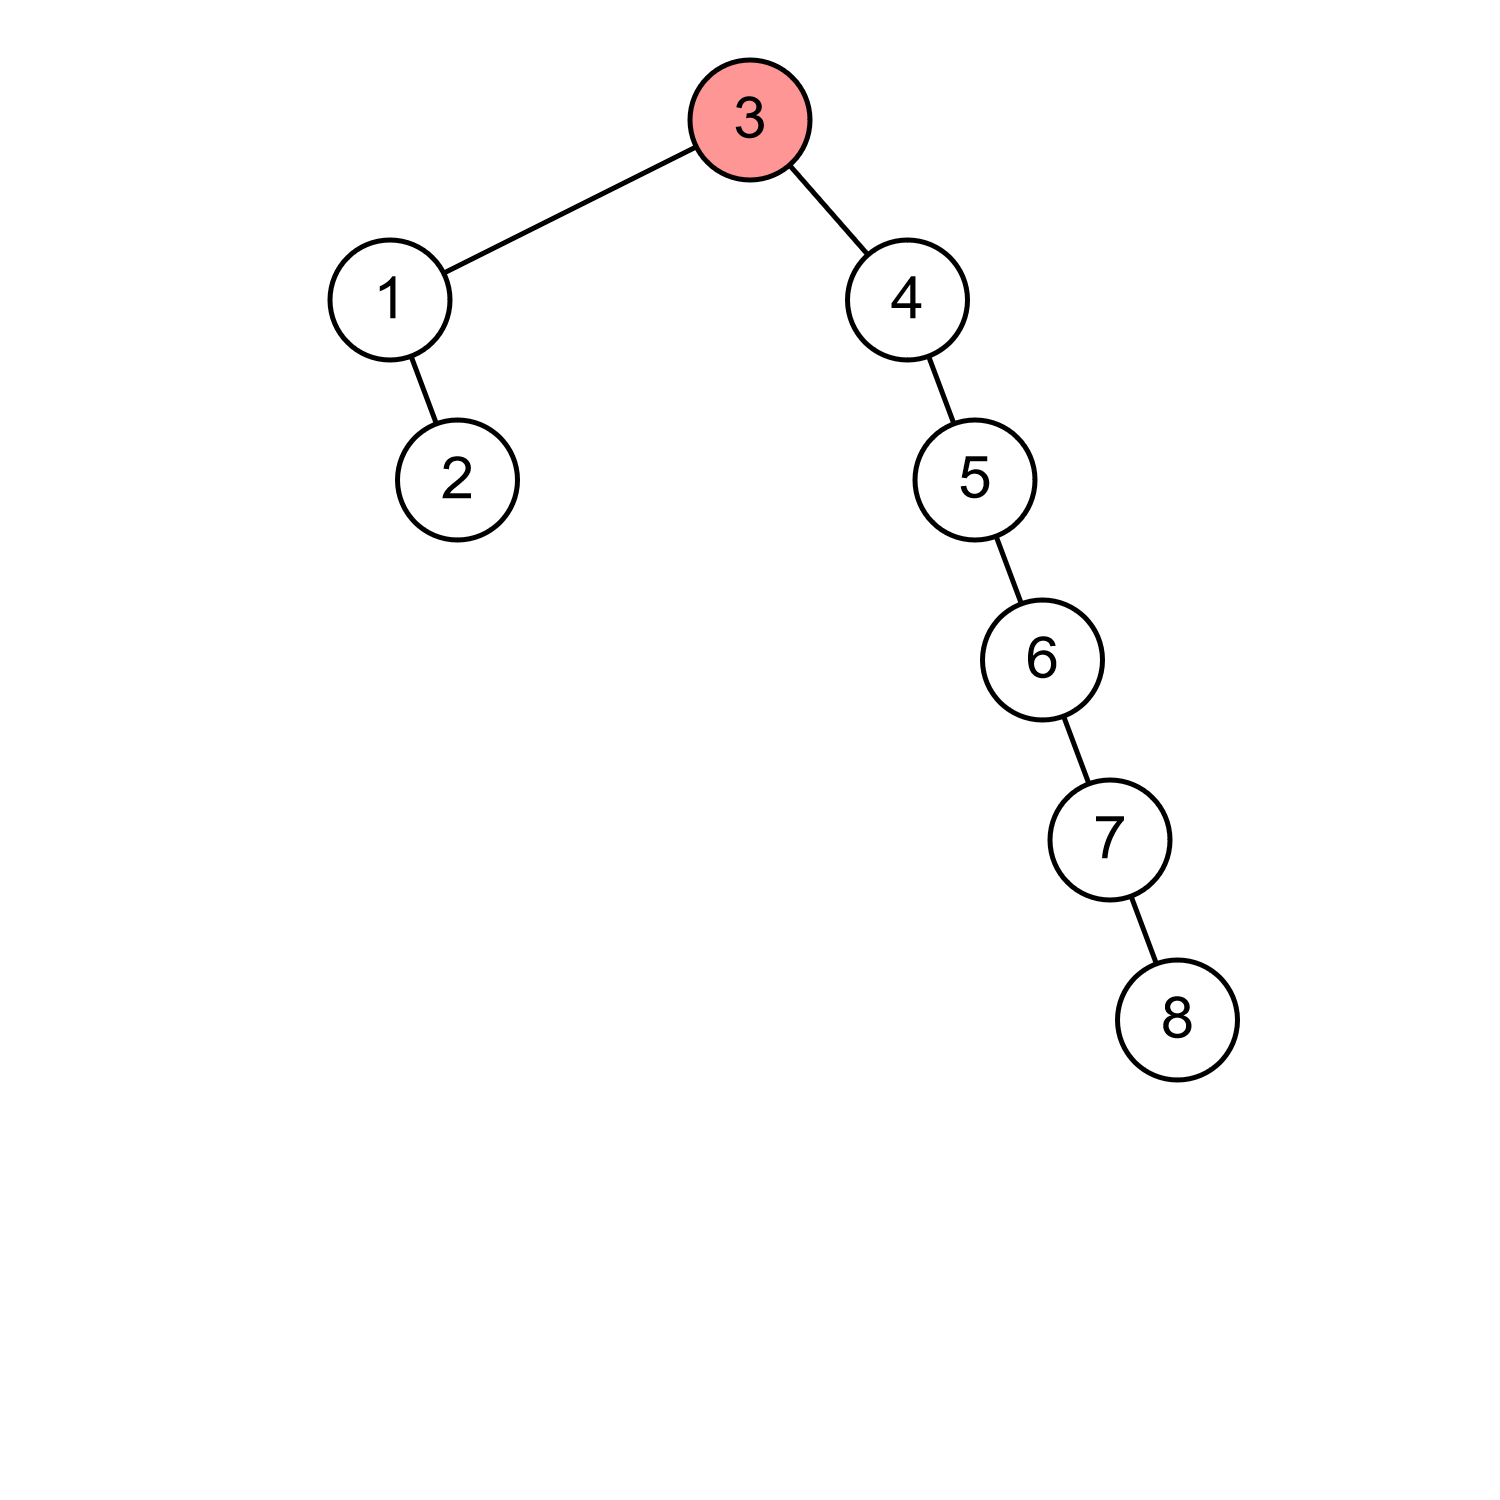
\includegraphics[width=\textwidth]{img/1b/5}
            \end{subfigure}
            \begin{subfigure}[b]{0.23\textwidth}
                \centering
                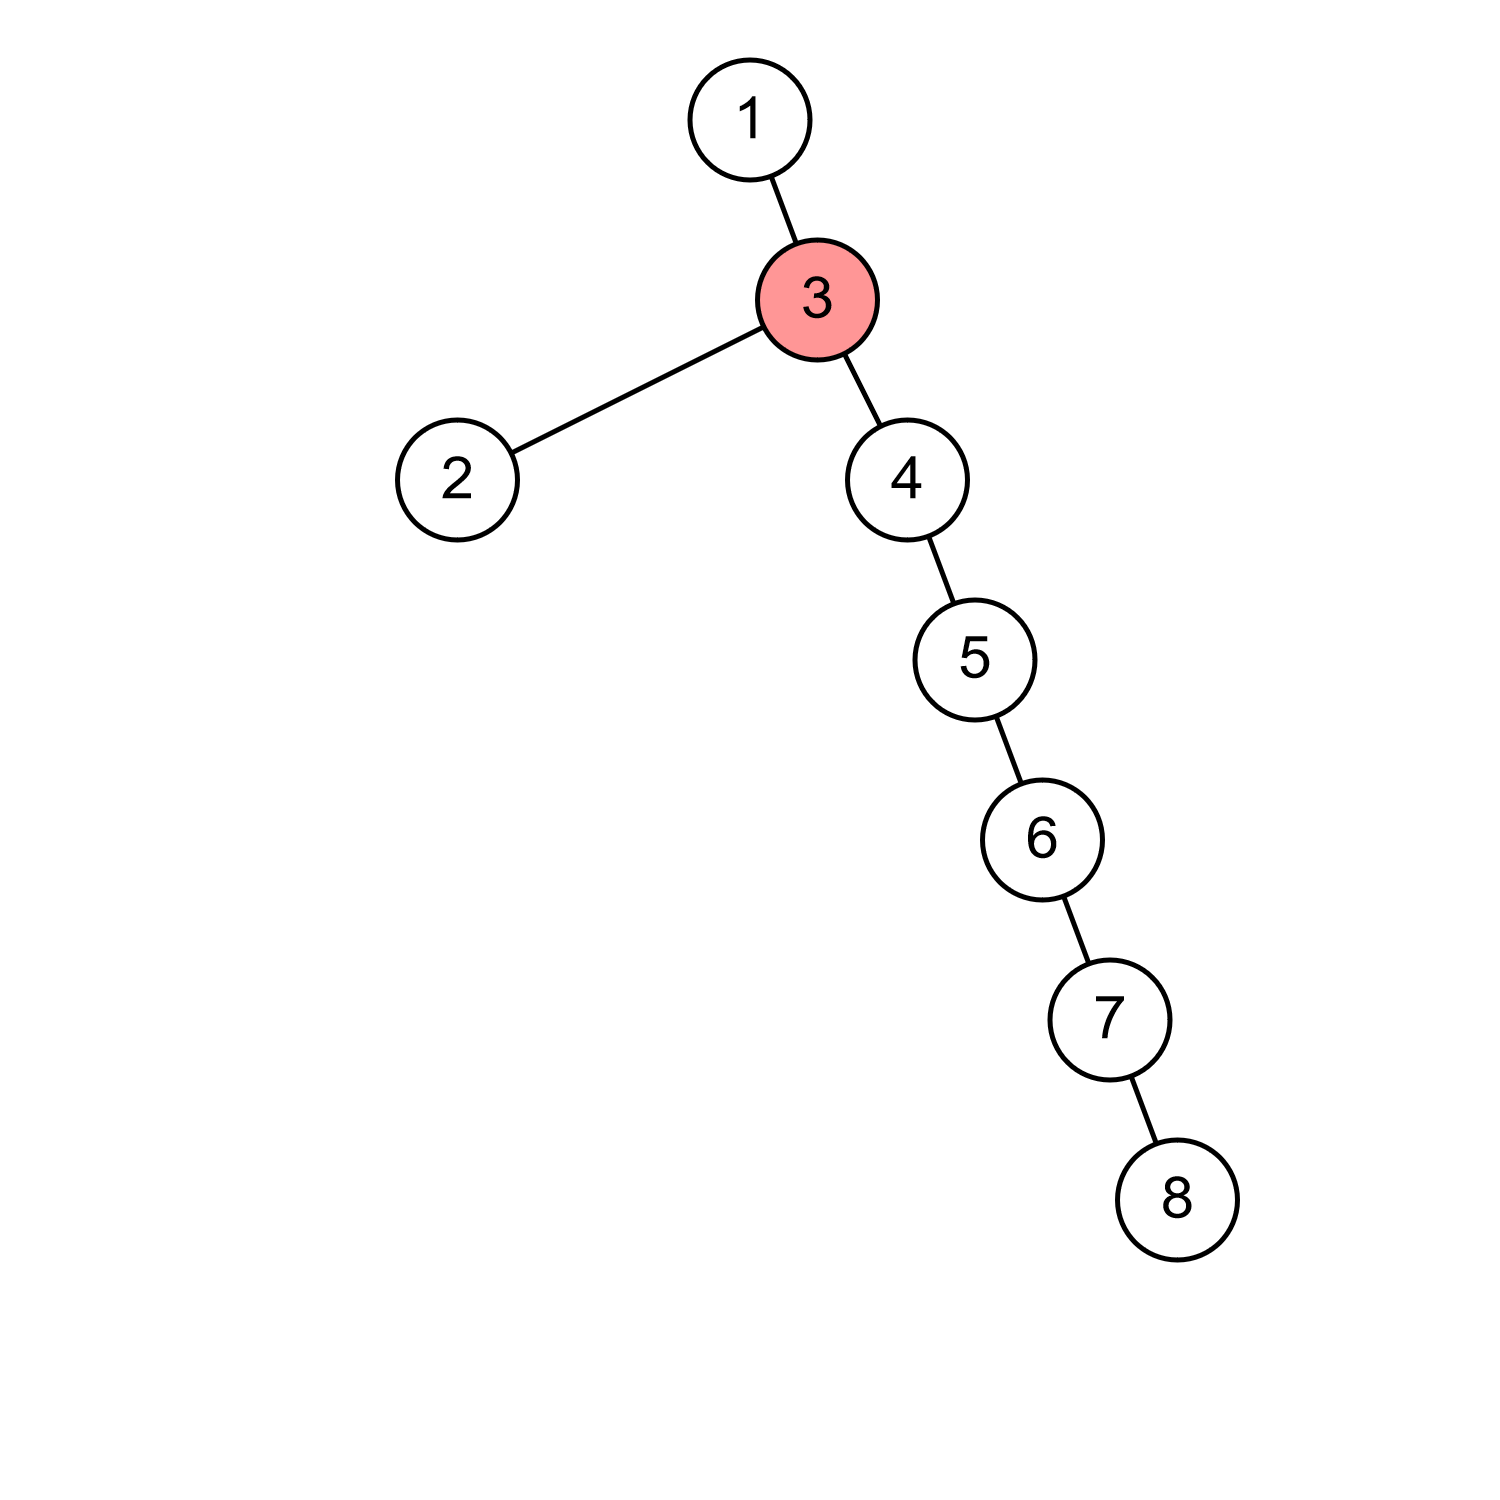
\includegraphics[width=\textwidth]{img/1b/6}
            \end{subfigure}
            \begin{subfigure}[b]{0.23\textwidth}
                \centering
                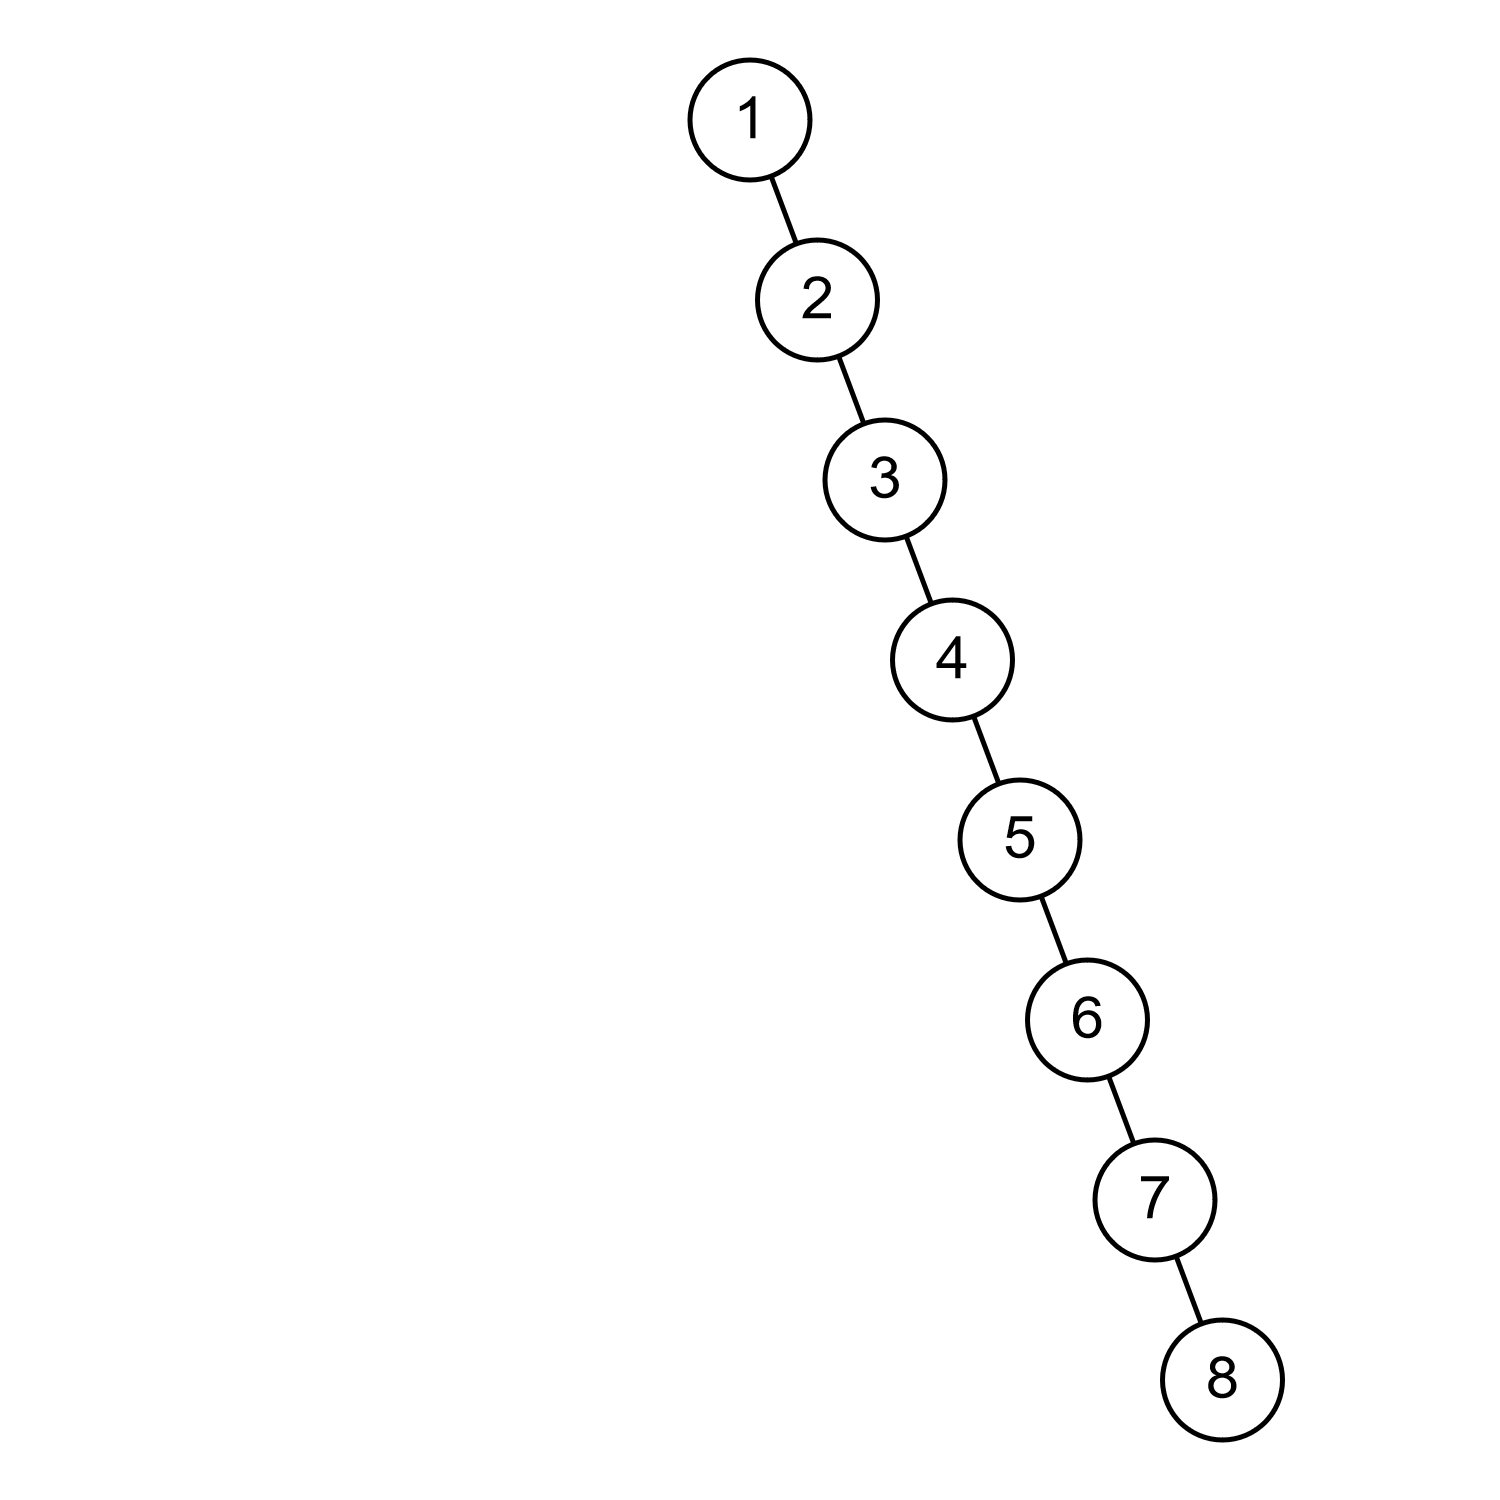
\includegraphics[width=\textwidth]{img/1b/7}
            \end{subfigure}
        \end{figure}
        \FloatBarrier

        Die Idee, um einen beliebigen Baum in einen entarteten zu konvertieren, ist, den entarteten Baum in der Achse von der Wurzel bis zum Maximum des Baumes aufzubauen (die Achse, die entsteht, wenn man von der Wurzel aus immer den rechten Nachfolger nimmt).
        Solange es noch Knoten gibt, die nicht in der Achse liegen, muss rotiert werden.
        Sobald eine Rechtsrotation auf einem Knoten der Achse durchgeführt wird, wird der linke Nachfolger des Knotens ebenfalls Teil der Achse.
        Alle bisherigen Knoten der Achse bleiben auch in der Achse.
        Mit jeder Rotation wird die Achse also um genau 1 länger.
        Im Worst-Case liegt zu Beginn allein der Wurzelknoten in der Achse.
        Somit sind dann $n - 1$ Rechtsrotationen nötig um die übrigen Knoten in die Achse einzusortieren.
    \end{enumerate}
\end{loesung}

\begin{aufgabe}{2}{Rot-Schwarz-Bäume}
    \begin{enumerate}
        \item
        Nennen Sie zwei Vorteile und zwei Nachteile von RS-Bäumen in der Praxis im Vergleich zu AVL-Bäumen.

        \item \hard Fügen Sie jeweils den Wert 7 in die folgenden RS-Bäume ein.
        Fügen Sie dafür einen roten Knoten mit Wert 7 an die entsprechende Stelle gemäß der Suchbaumeigenschaft in den Baum ein.
        Nutzen Sie anschließend jeweils die angegebenen Operationen, um alle RS-Baum-Eigenschaften wiederherzustellen.
        Wie sehen die Bäume am Ende aus?

        \begin{figure}[h!]
            \centering
            \begin{subfigure}[t]{0.28\textwidth}
                \centering
                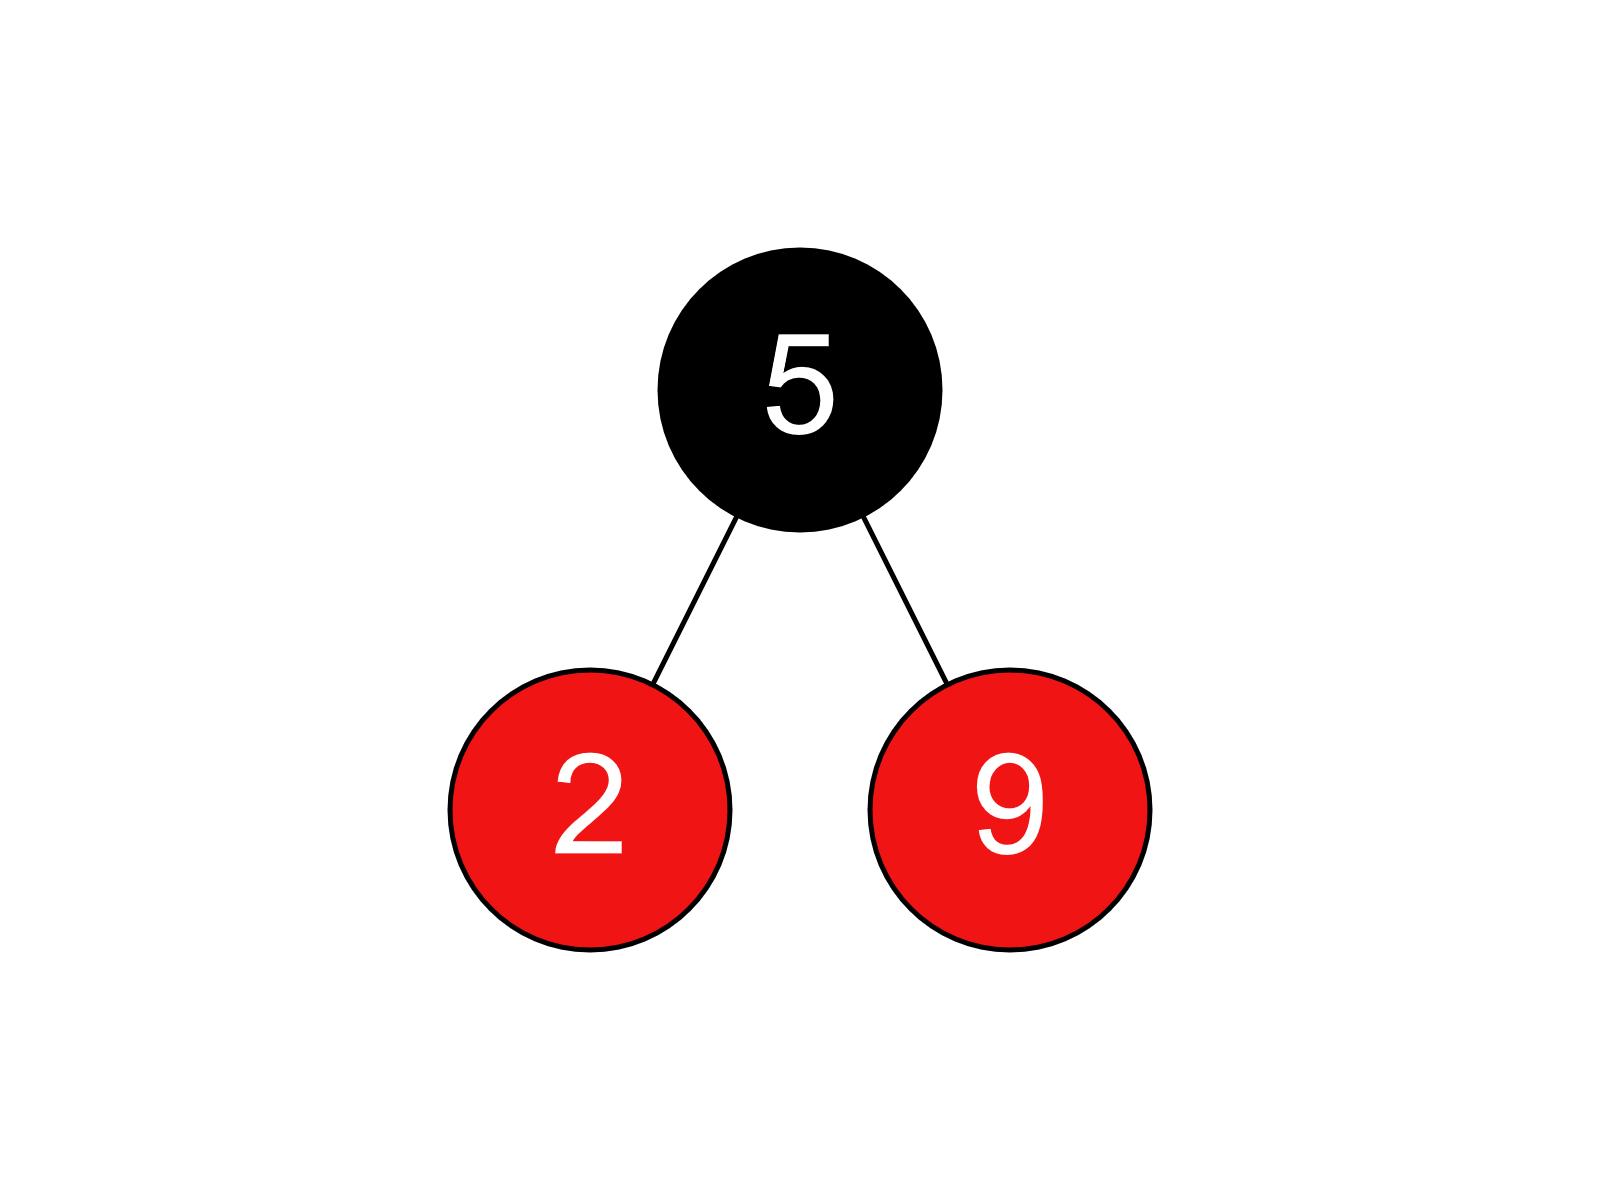
\includegraphics[width=0.6\textwidth]{img/2a_1}
                \caption*{i) Nach dem Einfügen 2 Knoten schwarz färben}
            \end{subfigure}
            \begin{subfigure}[t]{0.28\textwidth}
                \centering
                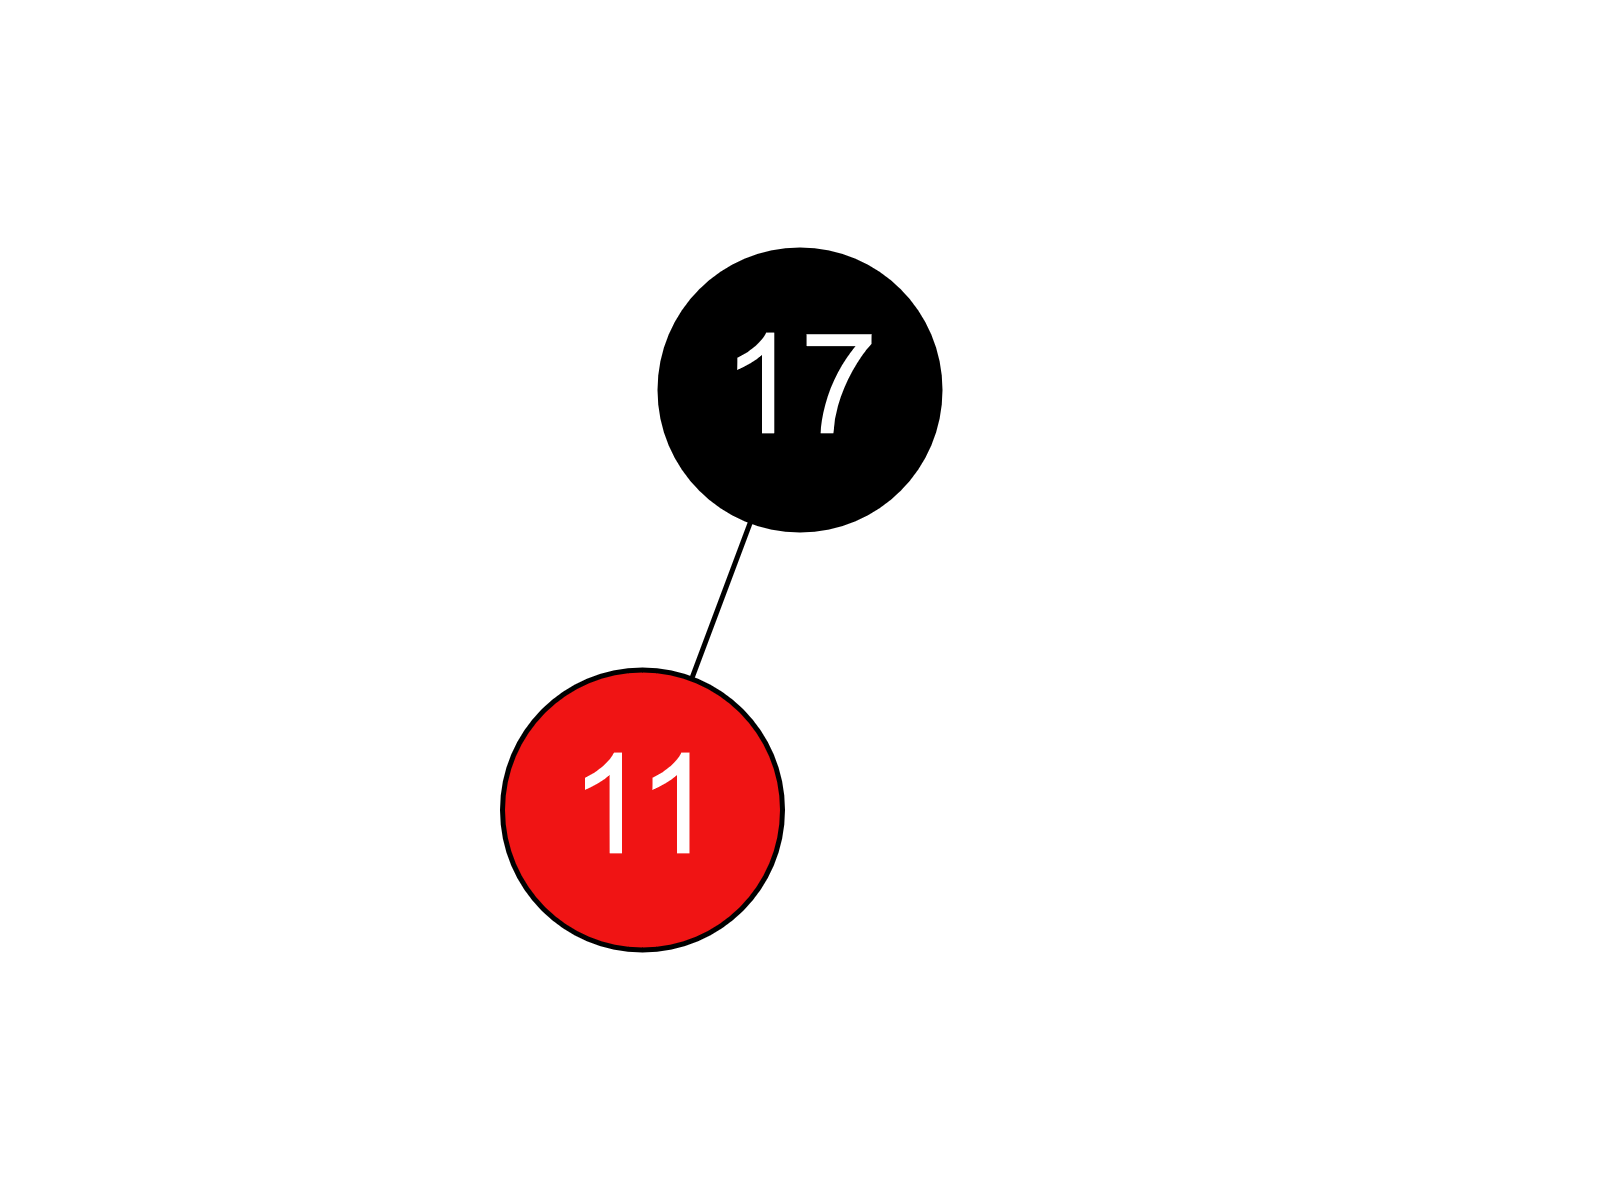
\includegraphics[width=0.6\textwidth]{img/2a_2}
                \caption*{ii) Nach dem Einfügen 1 Rotation durchführen, dann 1 Knoten rot und 1 schwarz färben}
            \end{subfigure}
            \begin{subfigure}[t]{0.28\textwidth}
                \centering
                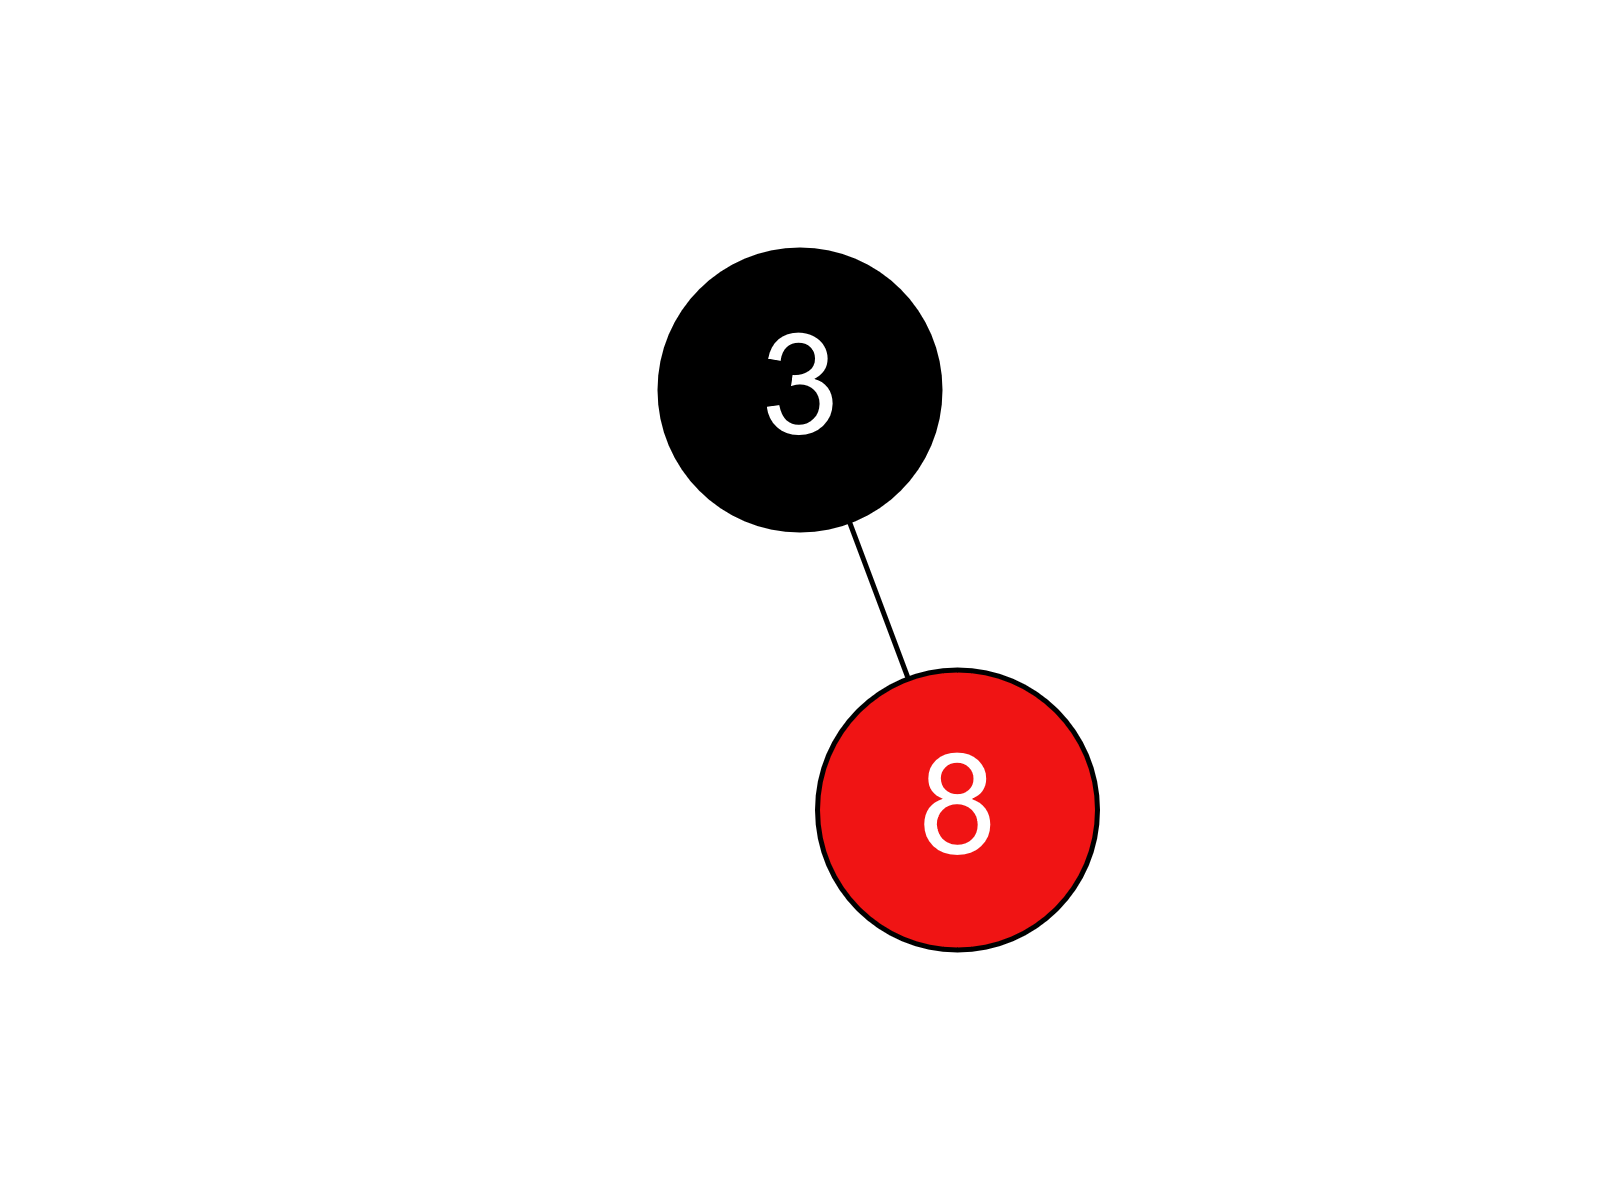
\includegraphics[width=0.6\textwidth]{img/2a_3}
                \caption*{iii) Nach dem Einfügen 2 Rotationen durchführen, dan 1 Knoten rot und 1 schwarz färben}
            \end{subfigure}
        \end{figure}
        \FloatBarrier

        \item Wie viele Werte sind in einem RS-Baum mit Schwarz-Höhe \emph{bh} mindestens gespeichert? Wie viele maximal?

        \item Beweisen oder widerlegen Sie folgende Behauptung: Bei jedem roten Knoten eines RS-Baumes sind entweder beide oder keiner der Nachfolger das RS-Blatt.

        \item \hard Wenn Sie in einem RS-Baum jeden schwarzen Knoten mit seinem/seinen roten Nachfolger(n) verschmelzen und die Nachfolger des roten Knotens als Nachfolger des schwarzen Knotens übernehmen, erhalten Sie einen Baum, mit potentiell mehr als einem Wert und mehr als zwei Nachfolgern pro Knoten.
        Beispiel:
        \begin{figure}[h!]
            \centering
            \begin{subfigure}[c]{0.2\textwidth}
                \centering
                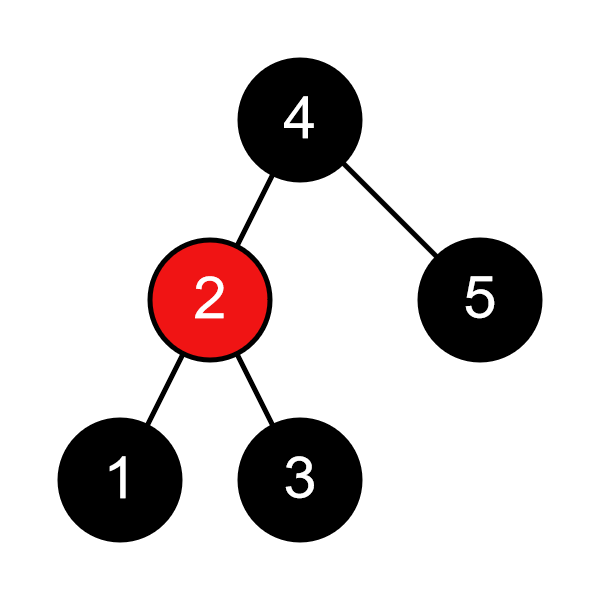
\includegraphics[width=0.6\textwidth]{img/2d_1}
            \end{subfigure}
            $\rightarrow$
            \begin{subfigure}[c]{0.2\textwidth}
                \centering
                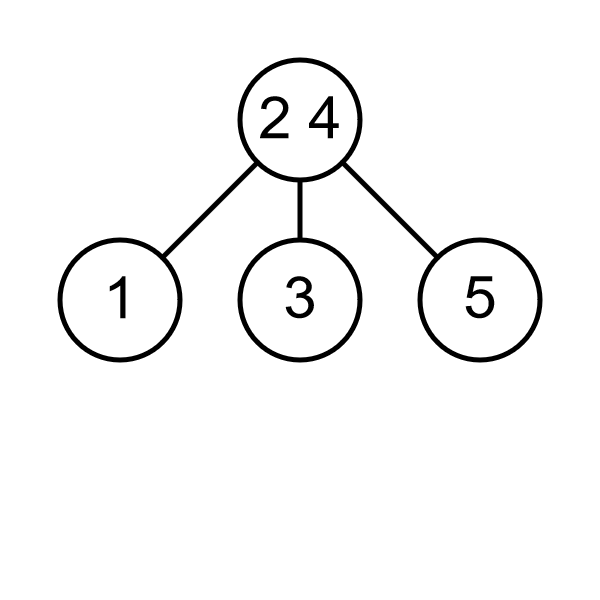
\includegraphics[width=0.6\textwidth]{img/2d_2}
            \end{subfigure}
        \end{figure}
        \FloatBarrier
        Welche Art von Baum aus der Vorlesung erhalten Sie?
        Welchen Baum erhalten Sie, wenn Sie beim folgenden RS-Baum jeden schwarzen Knoten mit seinem/seinen roten Nachfolger(n) verschmelzen?
        \begin{figure}[h!]
            \centering
            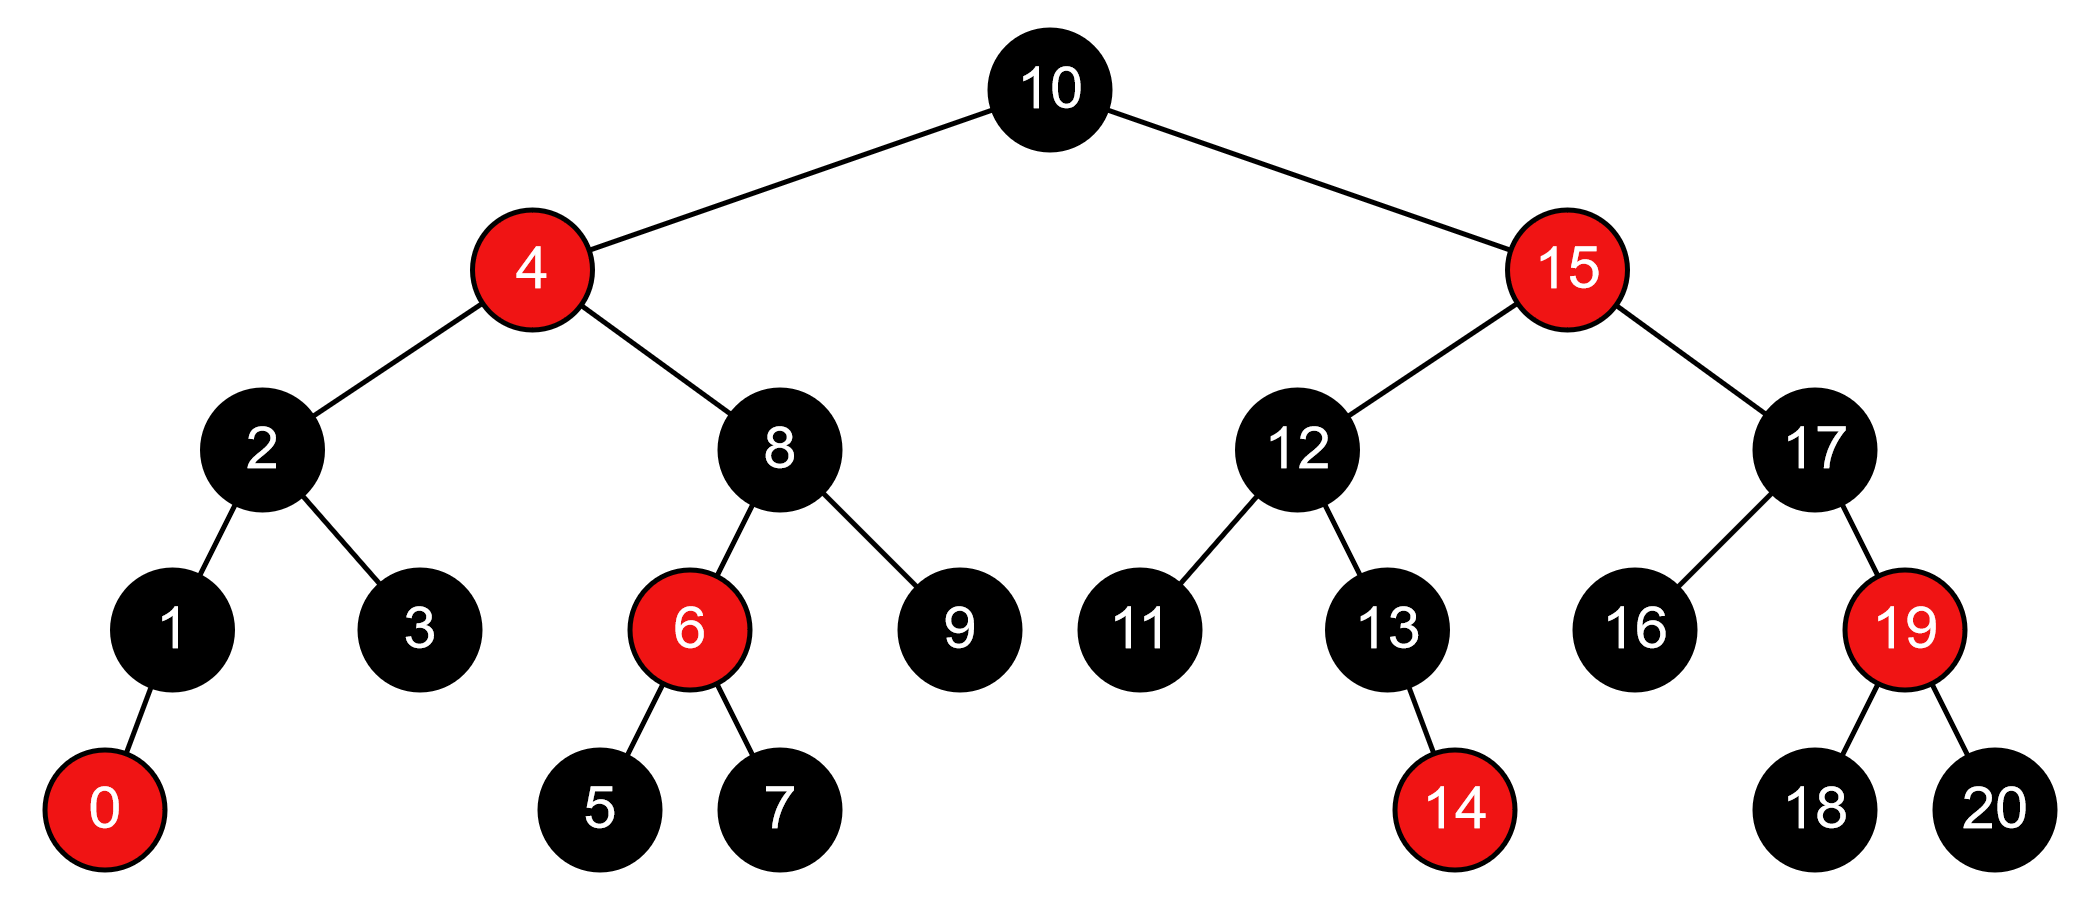
\includegraphics[width=0.5\textwidth]{img/2d}
        \end{figure}
        \FloatBarrier
        Welche Art von Bäumen erhalten Sie allgemein, wenn Sie die obige Transformation bei RS-Bäumen durchführen.
        Begründen Sie Ihre Antwort?
    \end{enumerate}
    
\end{aufgabe}
\begin{loesung}
    \begin{enumerate}[label=\alph*)]
        \item
        Allgemein gilt: AVL-Bäume sind strenger balanciert als RS-Bäume (maximal ca. 1.45 Mal so hoch wie der optimale Baum vs. maximal 2 Mal so hoch).

        \textbf{Vorteile:}
        \begin{itemize}
            \item Schnelleres Einfügen und Löschen, da aufgrund der weniger strengen Balancierung weniger Rotationen erforderlich sind, um den Baum wieder auszubalancieren.
            Insbesondere sind bei AVL-Bäumen beim Löschen bis zu $O(\log n)$ Rotationen erforderlich, bei RS-Bäumen nur konstant viele.
            \item Weniger zusätzlicher Speicherplatz pro Knoten erforderlich: 1 Bit (rot/schwarz) vs. die Höhe. \newline
            \emph{Anmerkung}: beim AVL-Baum gibt es nur drei relevante Fälle, die unterschieden werden: links 1 höher, gleich hoch, rechts 1 höher.
            Daher reichen eigentlich nur 2 zusätzliche Bits aus, um den jeweiligen Fall pro Knoten abzuspeichern.
            \item Der Geschwindigkeitsvorteil von AVL-Bäumen durch die niedrigeren Bäume ist in der Praxis häufig vernachlässigbar.
        \end{itemize}
        \textbf{Nachteile:}
        \begin{itemize}
            \item Langsameres Suchen: RS-Bäume sind schlechter ausbalanciert als AVL-Bäume und damit im Allgemeinen höher.

            \item Mehr unterschiedliche Fälle zu berücksichtigen:
            Bei AVL-Bäumen reicht es aus, die Höhe der Nachfolger und bei AVL-Verstoß noch der Höhe zweier Enkelknoten zu vergleichen.
            Bei RS-Bäumen gibt es je nach Farbe der benachbarten Knoten  weitere Fälle, die jeweils unterschiedlich behandelt werden müssen.

            \item Weniger intuitiv: Es ergibt intuitiv Sinn, wie die AVL-Eigenschaft zu balancierten Bäumen führt und wie Abweichungen durch Rotationen behoben werden können.
            Bei RS-Bäumen ist der Sinn der einzelnen Eigenschaften nicht sofort klar und auch Abweichungen sind nicht so intuitiv zu beheben.
        \end{itemize}
    
        \item 
        \begin{enumerate}[label=\roman*)]
            \item \ \\
            \begin{figure}[h!]
                \centering
                \begin{subfigure}[t]{0.15\textwidth}
                    \centering
                    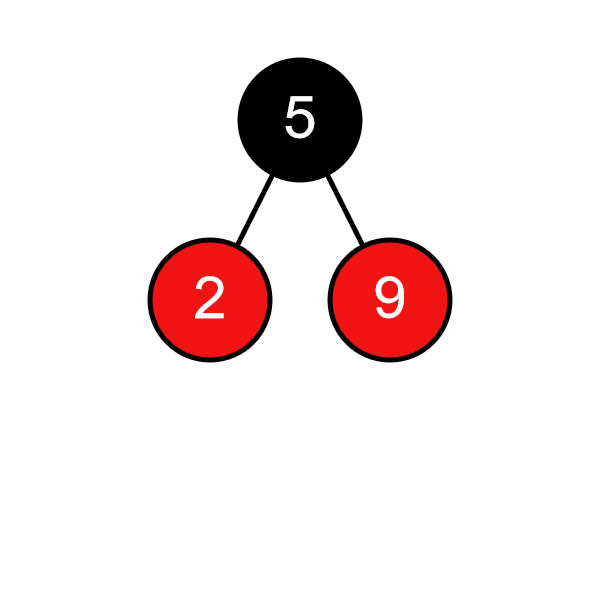
\includegraphics[width=\textwidth]{img/2b/1}
                \end{subfigure}
                \begin{subfigure}[t]{0.15\textwidth}
                    \centering
                    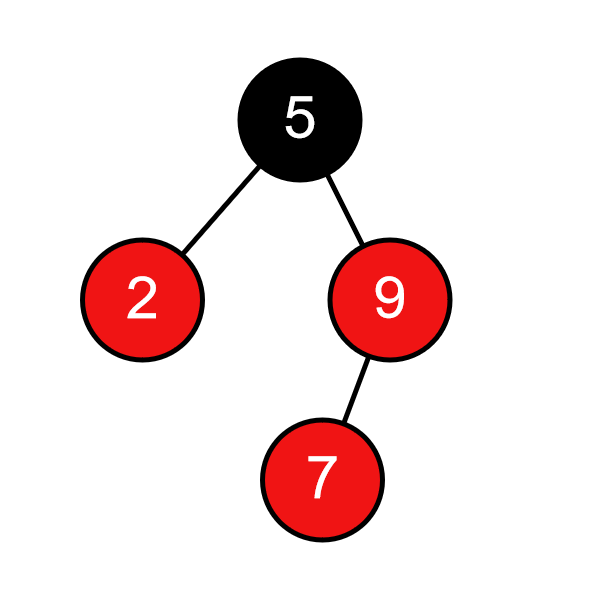
\includegraphics[width=\textwidth]{img/2b/2}
                \end{subfigure}
                \begin{subfigure}[t]{0.15\textwidth}
                    \centering
                    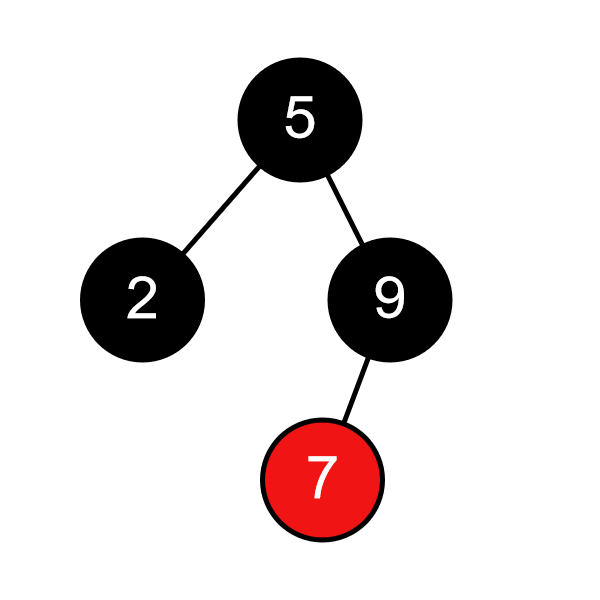
\includegraphics[width=\textwidth]{img/2b/3}
                \end{subfigure}
            \end{figure}
            \FloatBarrier
            \item \ \\
            \begin{figure}[h!]
                \centering
                \begin{subfigure}[t]{0.15\textwidth}
                    \centering
                    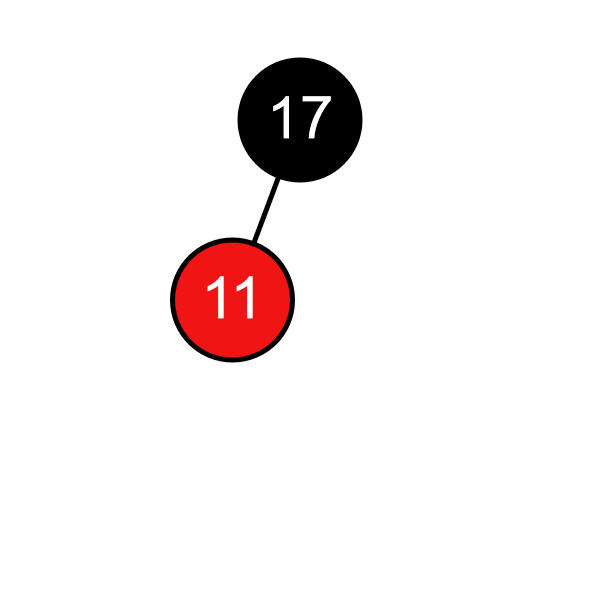
\includegraphics[width=\textwidth]{img/2b/4}
                \end{subfigure}
                \begin{subfigure}[t]{0.15\textwidth}
                    \centering
                    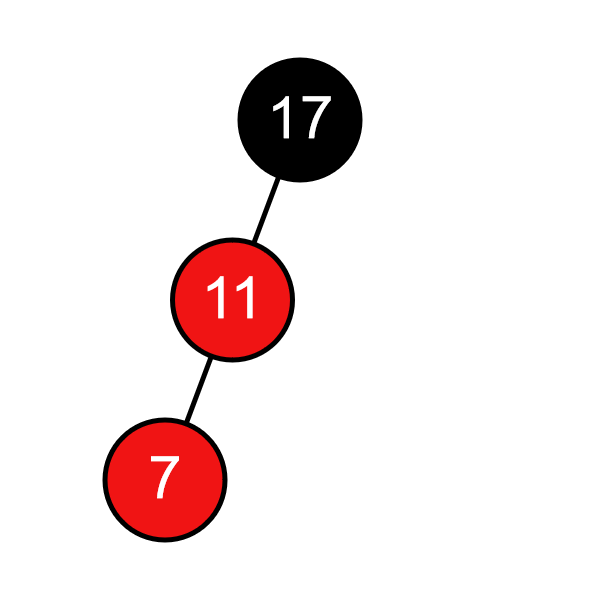
\includegraphics[width=\textwidth]{img/2b/5}
                \end{subfigure}
                \begin{subfigure}[t]{0.15\textwidth}
                    \centering
                    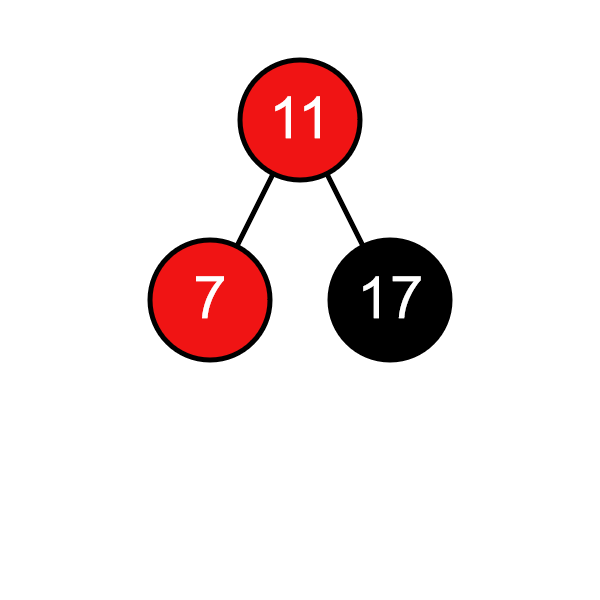
\includegraphics[width=\textwidth]{img/2b/6}
                \end{subfigure}
                \begin{subfigure}[t]{0.15\textwidth}
                    \centering
                    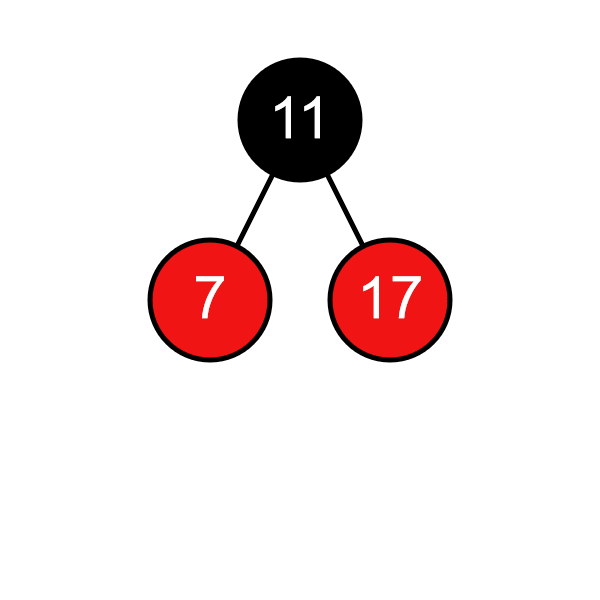
\includegraphics[width=\textwidth]{img/2b/7}
                \end{subfigure}
            \end{figure}
            \item \ \\
            \begin{figure}[h!]
                \centering
                \begin{subfigure}[t]{0.15\textwidth}
                    \centering
                    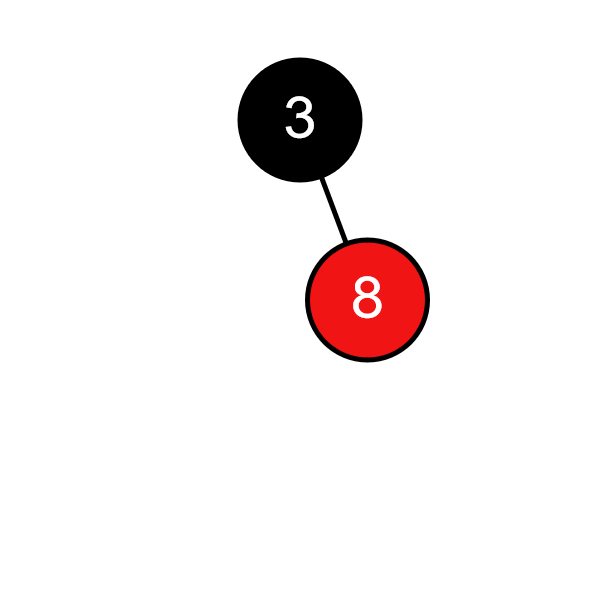
\includegraphics[width=\textwidth]{img/2b/8}
                \end{subfigure}
                \begin{subfigure}[t]{0.15\textwidth}
                    \centering
                    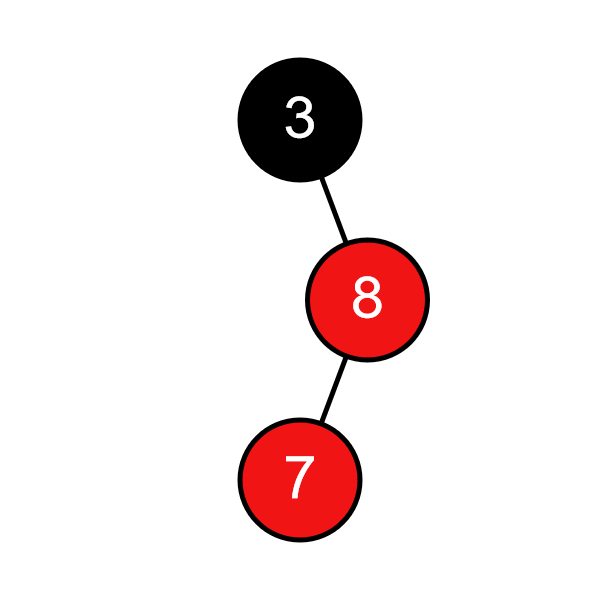
\includegraphics[width=\textwidth]{img/2b/10}
                \end{subfigure}
                \begin{subfigure}[t]{0.15\textwidth}
                    \centering
                    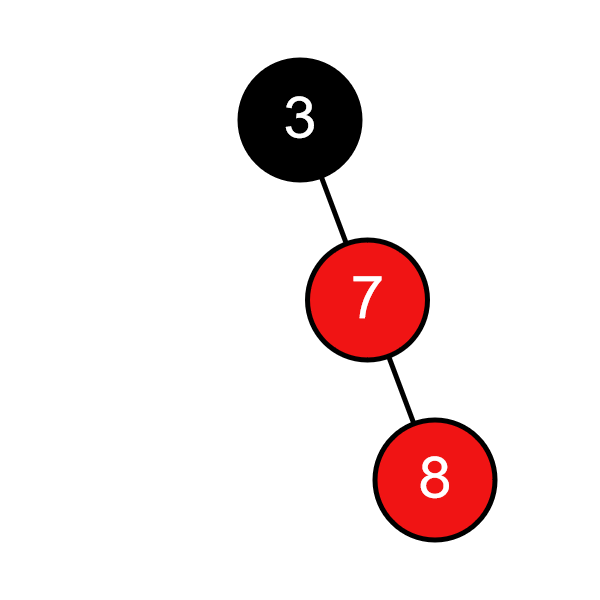
\includegraphics[width=\textwidth]{img/2b/11}
                \end{subfigure}
                \begin{subfigure}[t]{0.15\textwidth}
                    \centering
                    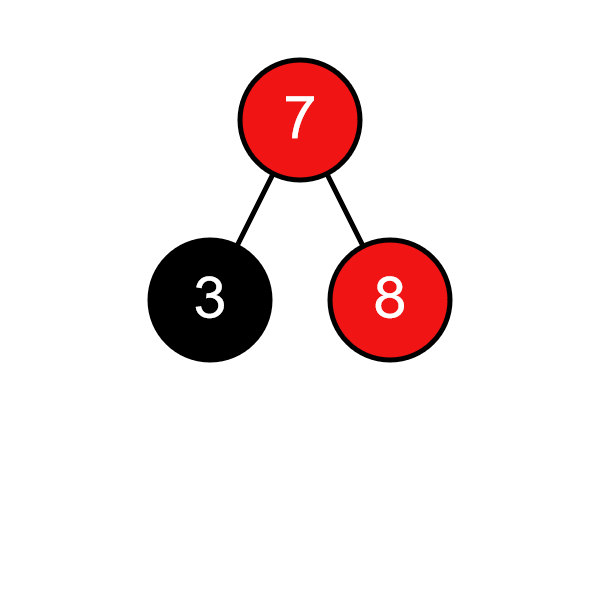
\includegraphics[width=\textwidth]{img/2b/12}
                \end{subfigure}
                \begin{subfigure}[t]{0.15\textwidth}
                    \centering
                    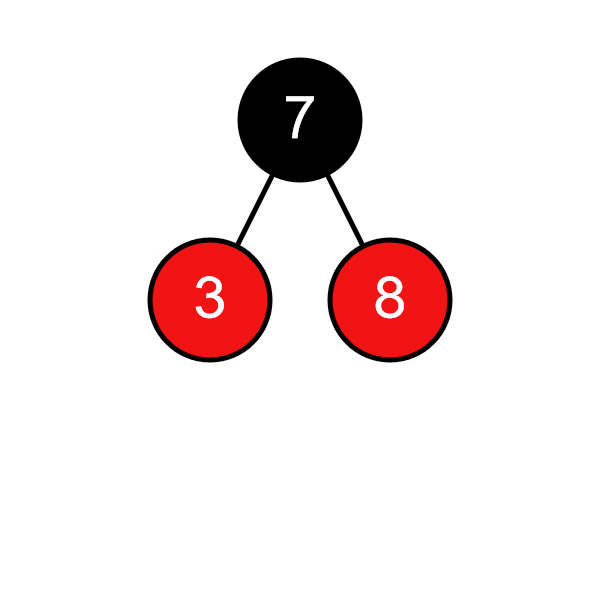
\includegraphics[width=\textwidth]{img/2b/13}
                \end{subfigure}
            \end{figure}
        \end{enumerate}
        Diese Operationen entsprechen den tatsächlichen drei Fällen, wie die RS-Eigenschaften beim Einfügen in der Praxis wiederhergestellt werden.
        
        \item
        Im Minimalfall enthält der Baum nur schwarze Knoten und ist damit so niedrig wie möglich.
        Der Baum entspricht dann einem vollständigen Binärbaum, da ja alle Pfade zu einem Blatt gleich viele schwarze Knoten beinhalten müssen.
        Die Höhe des Baumes entspricht der Schwarz-Höhe \emph{bh} (bei Bestimmen der Höhe wird ja die Wurzel nicht mit gezählt, dafür aber das RS-Blatt)
        Die Anzahl der Knoten in einem vollständigen Binärbaum mit Höhe \emph{bh} ist
        \begin{equation*}
            \sum\limits_{i = 0}^{\text{\emph{bh}}} 2^i \overset{\text{Geom. Reihe}}{=}
            2^{\text{\emph{bh}} + 1} - 1 = O(2^\text{\emph{bh}})
        \end{equation*}
        Im Maximalfall ist jeder Pfad von der Wurzel zu einem RS-Blatt abwechselnd schwarz und rot.
        Sowohl Wurzel und RS-Blatt sind gemäß der RS-Eigenschaften schwarz.
        Jeder Pfad muss also "schwarz", "rot", "schwarz", $\ldots$, "rot", "schwarz" eingefärbt sein.
        Daher sind alle Pfade von der Wurzel zum Blatt gleich lang, nämlich $2\text{\emph{bh}}$.
        Der RS-Baum entspricht also einem vollständigen Binärbaum mit Höhe $2\text{\emph{bh}}$.
        Analog zu oben enthält der Baum somit $2^{2\text{\emph{bh}} + 1} - 1 = O(4^\text{\emph{bh}})$ Knoten.

        \item Die Behauptung ist korrekt.
        \begin{proof}
            Beweis durch Widerspruch:
            Wenn ein roter Knoten weder zwei RS-Blätter noch zwei Nicht-RS-Blätter als Nachfolger hat, müssen seine Nachfolger genau ein RS-Blatt sowie ein anderer schwarzer Knoten sein.
            Angenommen, ein roter Knoten hat o.B.d.A. als linken Nachfolger ein RS-Blatt und als rechten Nachfolger einen anderen schwarzen Knoten.
            Sei $s$ die Anzahl der schwarzen Knoten auf dem Pfad von der Wurzel zu diesem roten Knoten (die Wurzel nicht mitgezählt).
            Dann enhält der Pfad von der Wurzel zum linken Nachfolger des roten Knotens (dem RS-Blatt) $s + 1$ schwarze Knoten (zur Erinnerung: das RS-Blatt ist immer schwarz).
            Ein Pfad vom rechten Nachfolger des roten Knotens bis zu einem RS-Blatt enthält jedoch mit dem rechten Nachfolger selbst und dem RS-Blatt mindestens 2 schwarze Knoten.
            Somit enthält der gesamte Pfad von der Wurzel über den betrachteten roten Knoten und dessen rechten Nachfolger zu einem RS-Blatt mindestens $s + 2$ schwarze Knoten.
            Das ist im direkten Widerspruch zur RS-Eigenschaft, dass jeder Pfad von der Wurzel zum Blatt gleich viele schwarze Knoten enthalten muss.
            Die getroffene Annahme ist also falsch und somit die Behauptung richtig.
        \end{proof}

        \item
        Der resultierende Baum ist ein B-Baum der Ordnung 3 oder 4 (da es Nicht-Wurzel-Knoten mit nur 1 Wert gibt).

        Der durchs Verschmelzen resultierende Baum sieht wie folgt aus:
        \begin{figure}[h!]
            \centering
            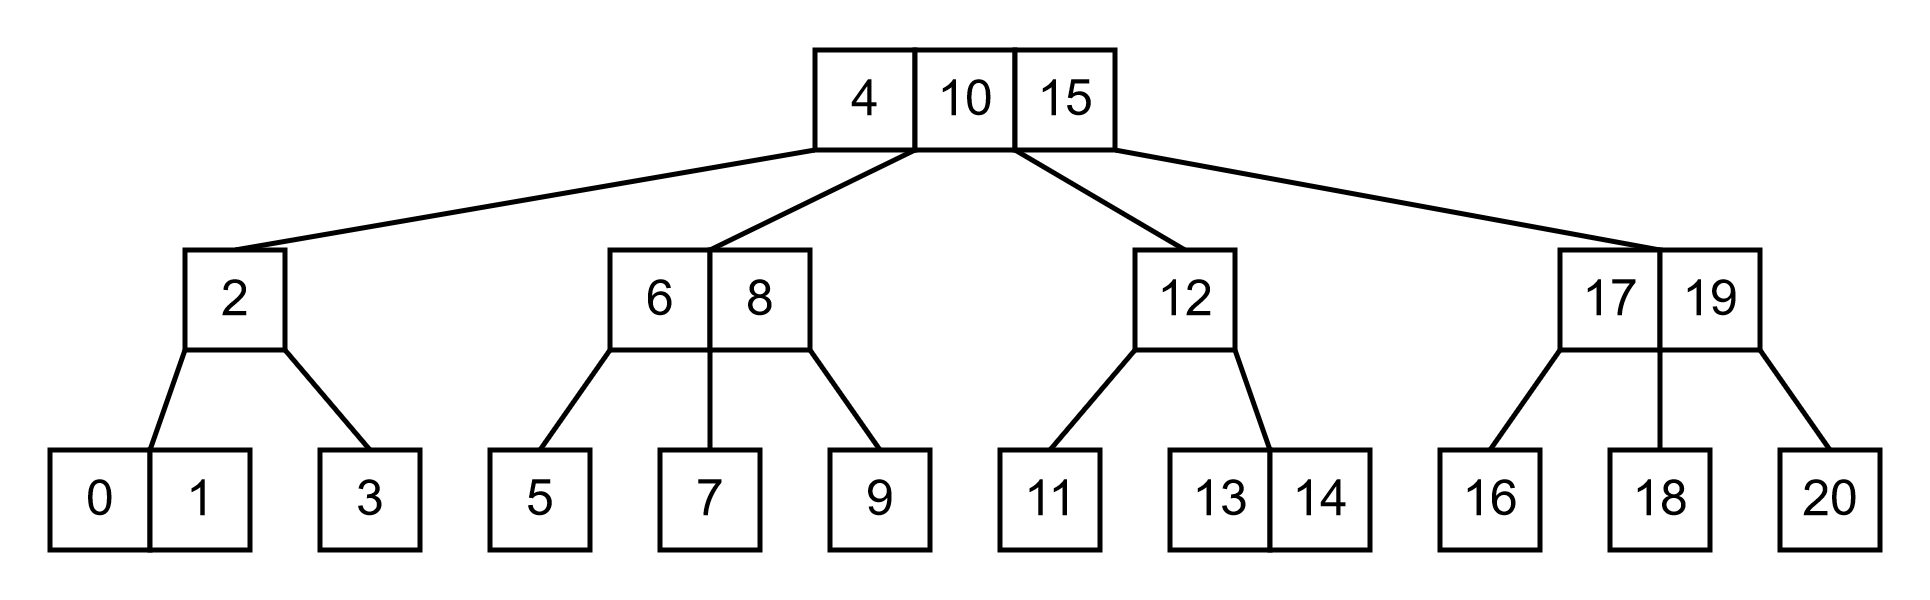
\includegraphics[width=0.5\textwidth]{img/2d_solution.png}
        \end{figure}
        \FloatBarrier

        Werden bei einem RS-Baum, wie in der Aufgabenstellung beschrieben, rote Knoten mit ihrem schwarzen Vorgänger verschmolzen und die verschiedenen Werte innerhalb eines Knotens nach dem Verschmelzen aufsteigend sortiert angeordnet, ist der resultierende Baum stets ein B-Baum der Ordnung 4.
        \begin{proof}
            Ein B-Baum der Ordnung 4 hat vier wesentliche Eigenschaften.
            Für alle Eigenschaften ist zu zeigen, dass der resultierende Baum beim Verschmelzen die entsprechende Eigenschaft besitzt:
            \begin{enumerate}[label=\arabic*.]
                \item \emph{Alle Blätter liegen in derselben Schicht.}
                In einem RS-Baum enthält jeder Pfad von der Wurzel zu einem RS-Blatt gleich viele schwarze Knoten.
                Da rote Knoten durch das Verschmelzen entfernt werden, aber die Pfade der schwarzen Knoten durch das Übernehmen der Nachfolger der roten Knoten im Wesentlichen erhalten bleiben, entspricht die Länge jedes Pfades von Wurzel zu Blattknoten im resultierenden Baum der Schwarz-Höhe des ursprünglichen Baumes.
                Daher sind alle Blätter gleich weit von der Wurzel entfernt und liegen somit auf der gleichen Schicht.
                \item \emph{Knoten mit Nachfolgern und $i$ Werten haben genau $i + 1$ Nachfolger.}
                Für schwarze Knoten gibt es beim Verschmelzen drei Fälle: der Knoten hat keinen, einen oder zwei rote Nachfolger.
                Es lässt sich leicht nachprüfen, dass die diese Eigenschaft in allen drei Fällen erfüllt ist.
                \item \emph{Alle Knoten außer der Wurzel haben mindestens 1 und maximal 3 Werte.}
                Wenn der ursprüngliche schwarze Knoten keinen roten Nachfolger hat, enthält der resultierende B-Baum-Knoten einen Wert; bei einem roten Nachfolger zwei Werte und bei zwei roten Nachfolgern drei Werte.
                \item \emph{Suchbaumeigenschaft.}
                Ohne einen formalen Beweis anzugeben, ist leicht zu sehen, dass auch diese Eigenschaft gilt.
                Beispiel: Im Baum aus der Aufgabenstellung ist der rechte Nachfolger der Wurzel (10) ein roter Knoten mit Wert 4.
                Das bedeutet, dass rechte Teilbaum von 4 nur Werte enthalten kann, die zwischen 4 und 10 liegen.
                Dieser Teilbaum korrespondiert direkt mit dem Teilbaum zwischen 4 und 10 im resultierenden B-Baum.
            \end{enumerate}
        \end{proof}
        Tatsächlich sind RS-Bäume isomorph (direkt ineinander konvertierbar) zu B-Bäumen der Ordnung 4. 
        Einfüge- und Löschoperationen der RS-Bäume verhalten sich direkt äquivalent zu den entsprechenden B-Baum-Operationen und umgekehrt.
    \end{enumerate}
\end{loesung}

\begin{aufgabe}{3}{B-Bäume}
    \begin{enumerate}[label=\alph*)]
        \item
        Nennen Sie zwei Vorteile und zwei Nachteile von B-Bäumen in der Praxis im Vergleich zu AVL-Bäumen.

        \item Geben Sie alle B-Bäume mit Ordnung 4 an, die genau die Werte 1, 3, 4, 5 und 7 enthalten.
        
        \item
        Gegeben sei folgender B-Baum der Ordnung 5:
        \begin{figure}[h!]
            \centering
            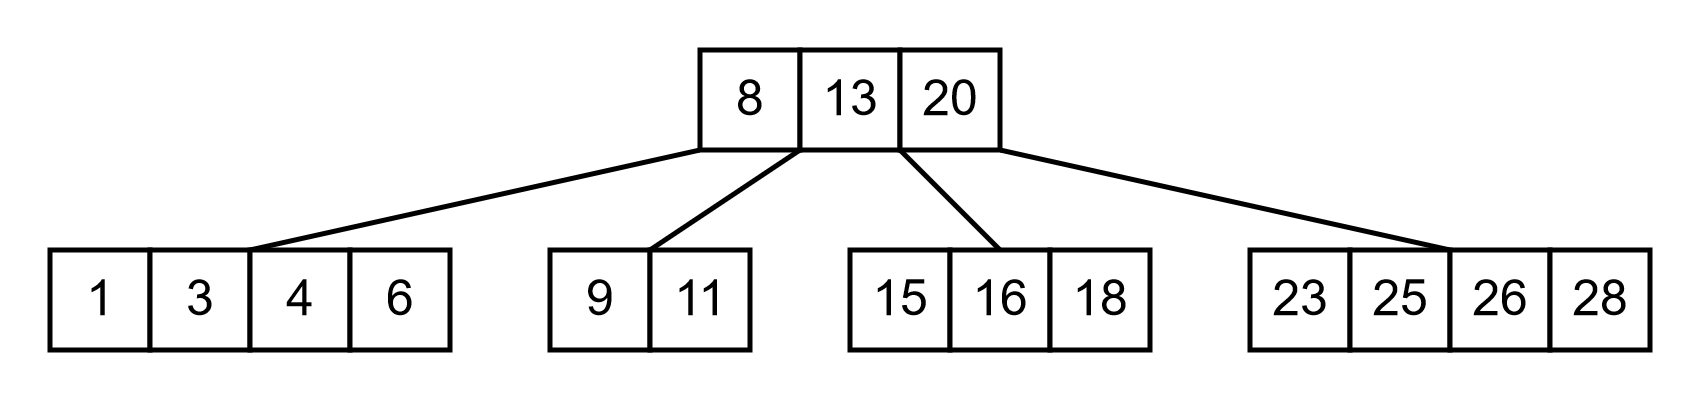
\includegraphics[width=0.5\textwidth]{img/3d}
        \end{figure}
        \FloatBarrier
        Führen Sie nacheinander folgende Operationen durch: 
        \textsc{Insert(2)}, \textsc{Remove(11)}, \textsc{Insert(7)}, \textsc{Insert(30)}, \textsc{Remove(8)}, \textsc{Remove(15)}.
        Geben Sie alle Zwischenschritte an.

        \item\label{b_tree_insert} Gegeben sei ein leerer B-Baum der Ordnung 4. Fügen Sie sukzessiv folgende Elemente in den Baum ein: 
        7, 3, 8, 18, 10, 14, 12, 13, 6, 15, 20.

        \item
        Entfernen Sie aus dem resultierenden Baum von Teilaufgabe \ref*{b_tree_insert} folgende Elemente:
        3, 13, 6, 18, 20, 10.

        \item \hard Angenommen, Sie haben einen B-Baum der Ordnung $t$ mit $n$ Werten im Arbeitsspeicher vorliegen:
        \begin{lstlisting}[language=c++]
class Node {
    int nValues; bool isLeaf;
    int values[t - 1]; Node *succ[t];
}
        \end{lstlisting}
        Implementieren Sie die Suchoperation, die überprüft, ob ein bestimmter Wert im Baum enthalten ist, in Pseudocode oder einer Programmiersprache Ihrer Wahl, einmal mit linearer Suche innerhalb eines Knotens und einmal mit binärer Suche.

        \item \hard Geben Sie die Worst-Case-Laufzeiten der beiden Algorithmen der vorherigen Teilaufgabe abhängig von $t$ und $n$ an.
    \end{enumerate}
\end{aufgabe}

\begin{loesung}
    \begin{enumerate}
        \item
        \textbf{Vorteile:}
        \begin{itemize}
            \item Wenn Knoten auf einem langsamen Speichermedium wie einer Festplatte gepspeichert werden, dann sind weniger Speicherzugriffe nötig, da der Baum weniger Knoten besitzt.
            \item B-Bäume, die im Arbeitsspeicher vorliegen, haben tendenziell ein besseres Cache-Verhalten als AVL-Bäume, da Werte einzelner Knoten in einem AVL-Baum weit weg voneinander im Arbeitsspeicher liegen können.
            Werte innerhalb eines B-Baum-Knotens liegen dagegen nah zusammen und werden typischerweise auf einmal in den Cache geladen.
            \item B-Bäume im Arbeitsspeicher benötigen weniger (häufig langsame) Speicherallokationen als AVL-Bäume.
            Bei AVL-Bäumen muss bei jedem Einfügen Speicher für den neuen Knoten allokiert werden, bei B-Bäumen nur wenn das entsprechende Blatt voll wird.
        \end{itemize}

        \textbf{Nachteile:}
        \begin{itemize}
            \item B-Bäume sind normalerweise schwieriger zu implementieren als AVL-Bäume.
            \item Wenn viele Knoten eines B-Baums minimal (also halb) besetzt sind, bleibt etwa die Hälfte des für den B-Baum verwendeten Speicherplatzes ungenutzt (Knoten werden normalerweise nicht dynamisch vergrößert, sondern in der vollen Größe initialisiert).
            \item B-Baum-Operationen sind typischerweise linear in der Ordnung des Baumes. Wenn die Ordnung groß ist (was sie in der Praxis oft ist), kann dies ein Performance-Nachteil gegenüber AVL-Bäumen sein.
        \end{itemize}

        \item \ \\
        \begin{figure}[h!]
            \centering
            \begin{subfigure}[b]{0.20\textwidth}
                \centering
                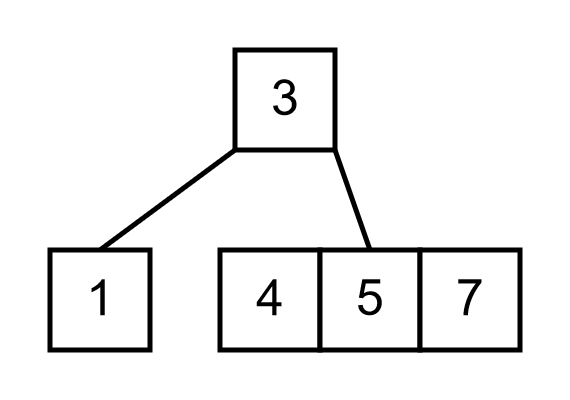
\includegraphics[width=\textwidth]{img/3b/1}
            \end{subfigure}
            \begin{subfigure}[b]{0.20\textwidth}
                \centering
                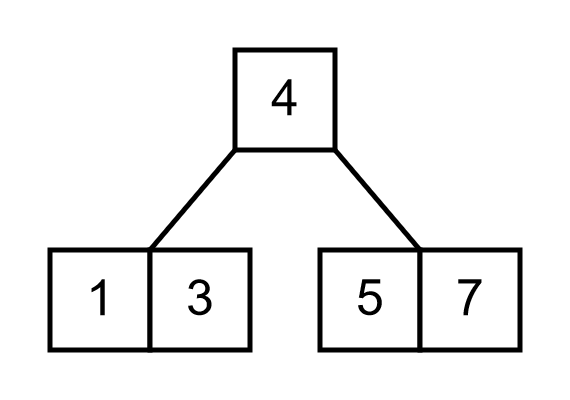
\includegraphics[width=\textwidth]{img/3b/2}
            \end{subfigure}
            \begin{subfigure}[b]{0.20\textwidth}
                \centering
                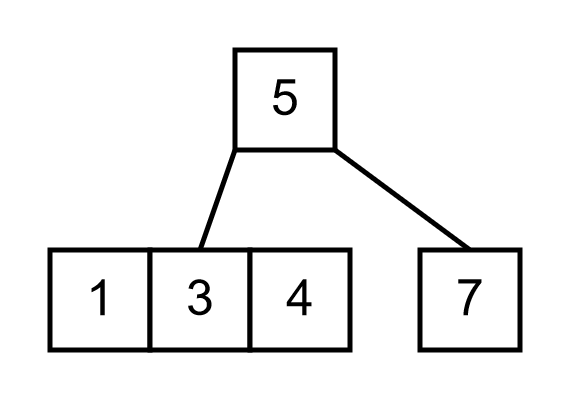
\includegraphics[width=\textwidth]{img/3b/3}
            \end{subfigure}
            \begin{subfigure}[b]{0.20\textwidth}
                \centering
                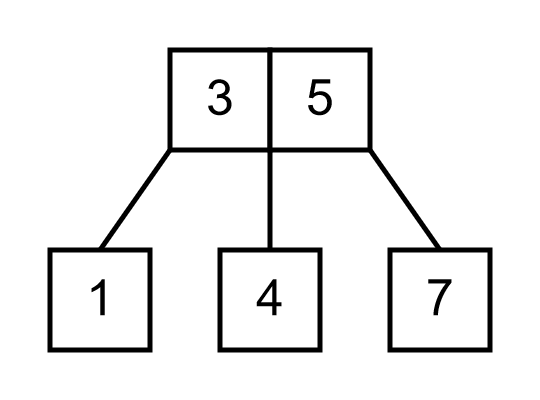
\includegraphics[width=\textwidth]{img/3b/4}
            \end{subfigure}
            \\
        \end{figure}
        \FloatBarrier

        \newpage
        \item \ \\
        \begin{figure}[h!]
            \centering
            \begin{subfigure}[b]{0.45\textwidth}
                \centering
                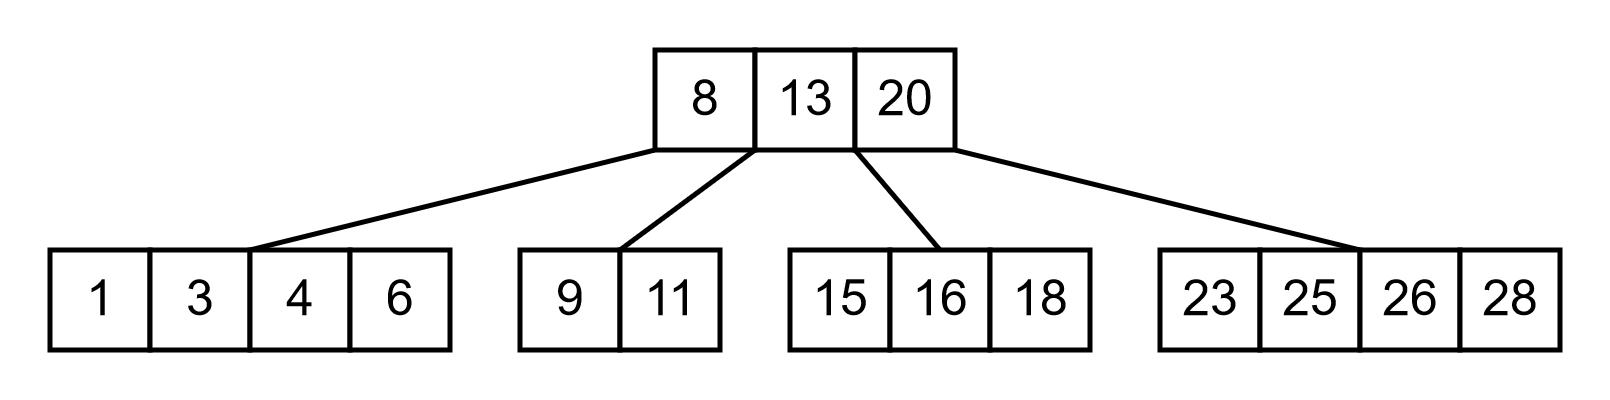
\includegraphics[width=\textwidth]{img/3c/1}
            \end{subfigure}
            \begin{subfigure}[b]{0.45\textwidth}
                \centering
                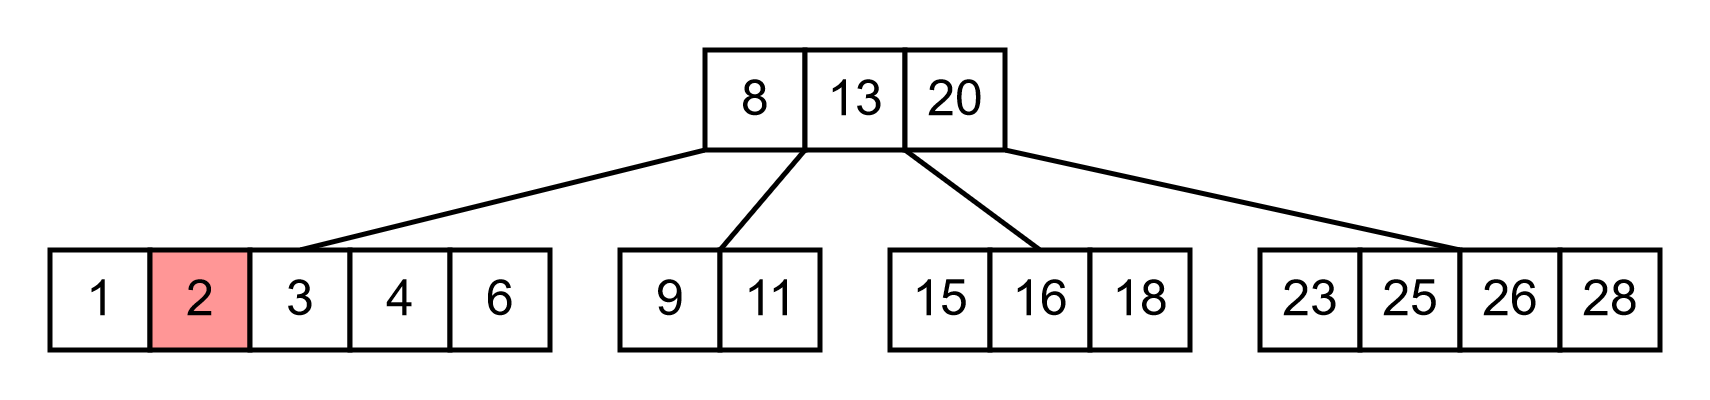
\includegraphics[width=\textwidth]{img/3c/2}
            \end{subfigure}
            \begin{subfigure}[b]{0.45\textwidth}
                \centering
                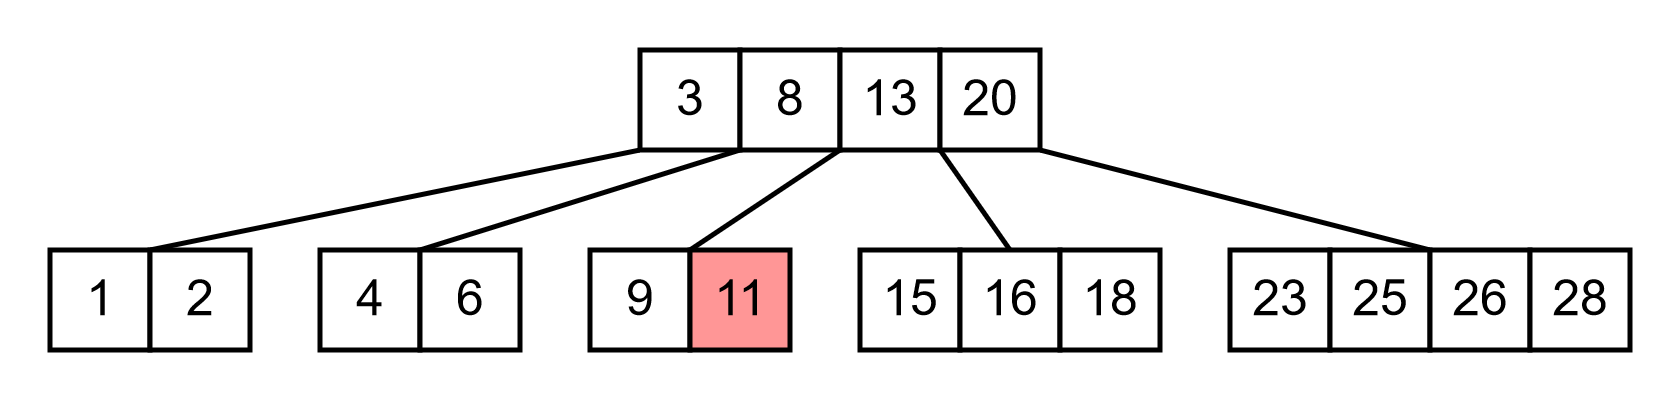
\includegraphics[width=\textwidth]{img/3c/3}
            \end{subfigure}
            \begin{subfigure}[b]{0.45\textwidth}
                \centering
                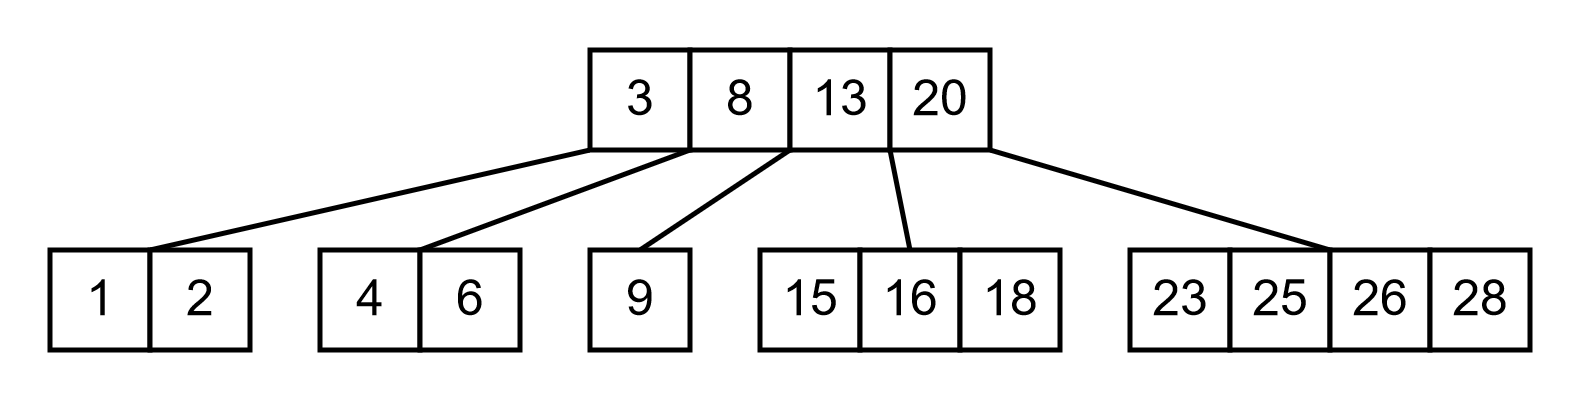
\includegraphics[width=\textwidth]{img/3c/3a}
            \end{subfigure}
            \begin{subfigure}[b]{0.45\textwidth}
                \centering
                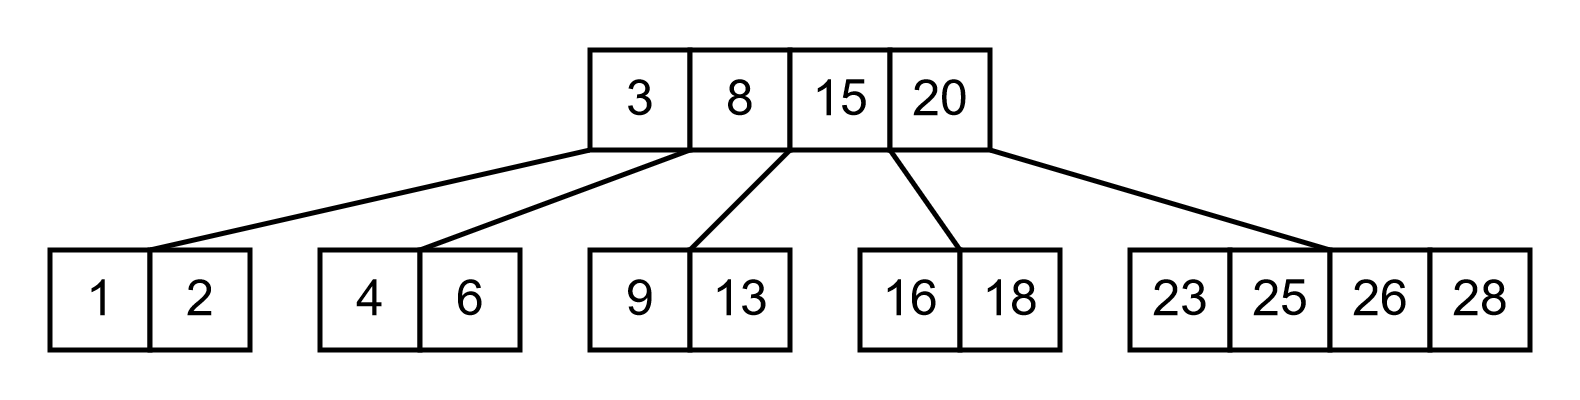
\includegraphics[width=\textwidth]{img/3c/4}
            \end{subfigure}
            \begin{subfigure}[b]{0.45\textwidth}
                \centering
                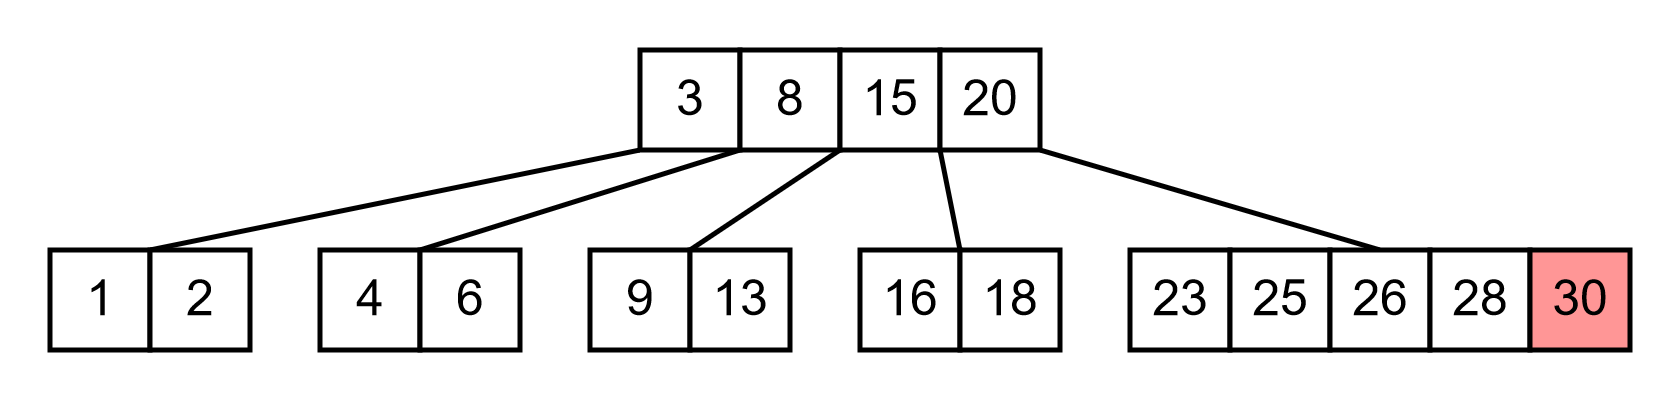
\includegraphics[width=\textwidth]{img/3c/5}
            \end{subfigure}
            \begin{subfigure}[b]{0.45\textwidth}
                \centering
                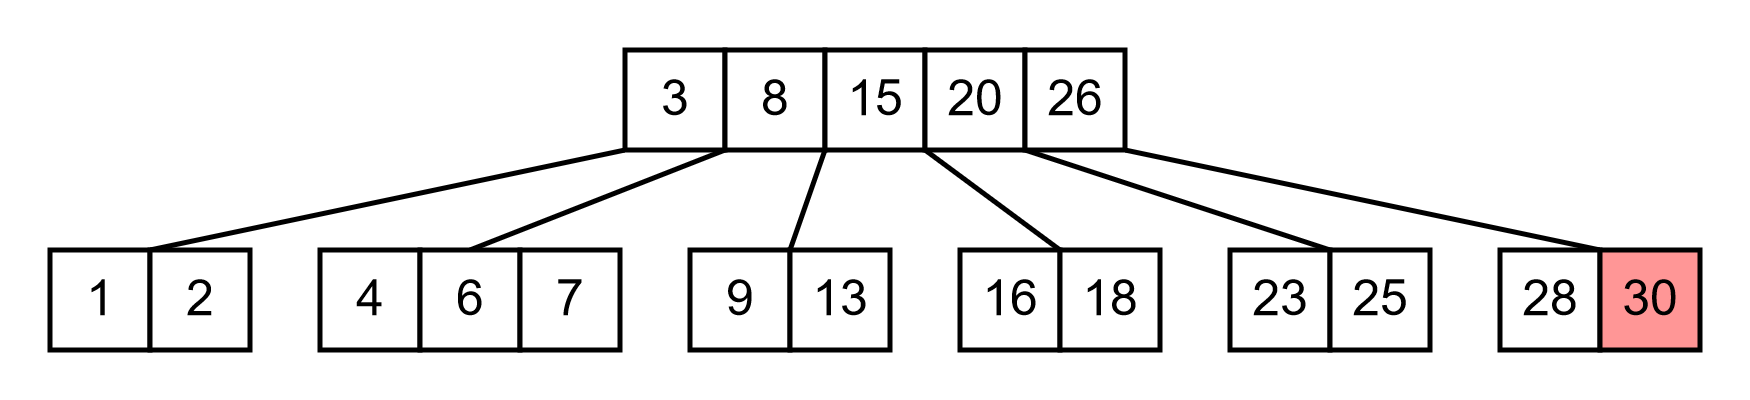
\includegraphics[width=\textwidth]{img/3c/6}
            \end{subfigure}
            \begin{subfigure}[b]{0.45\textwidth}
                \centering
                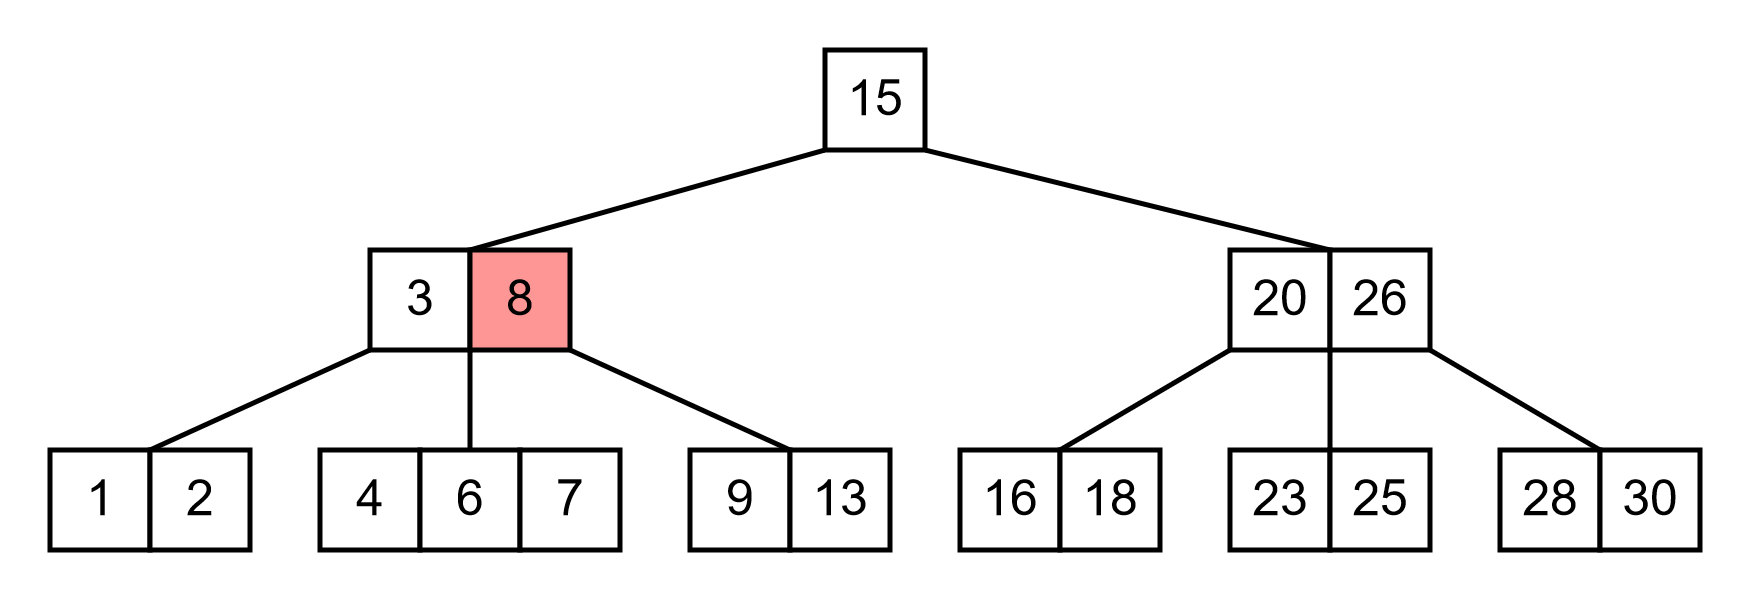
\includegraphics[width=\textwidth]{img/3c/7}
            \end{subfigure}
            \begin{subfigure}[b]{0.45\textwidth}
                \centering
                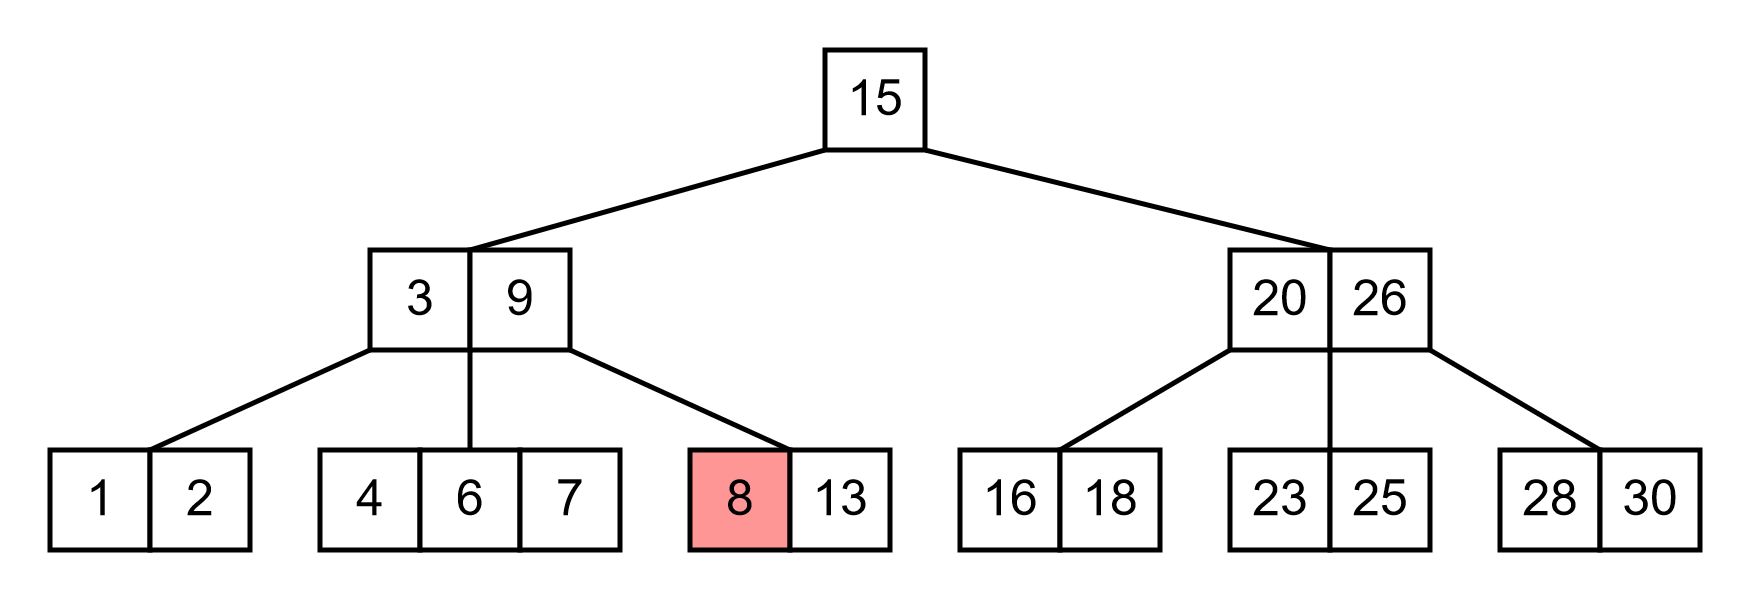
\includegraphics[width=\textwidth]{img/3c/8}
            \end{subfigure}
            \begin{subfigure}[b]{0.45\textwidth}
                \centering
                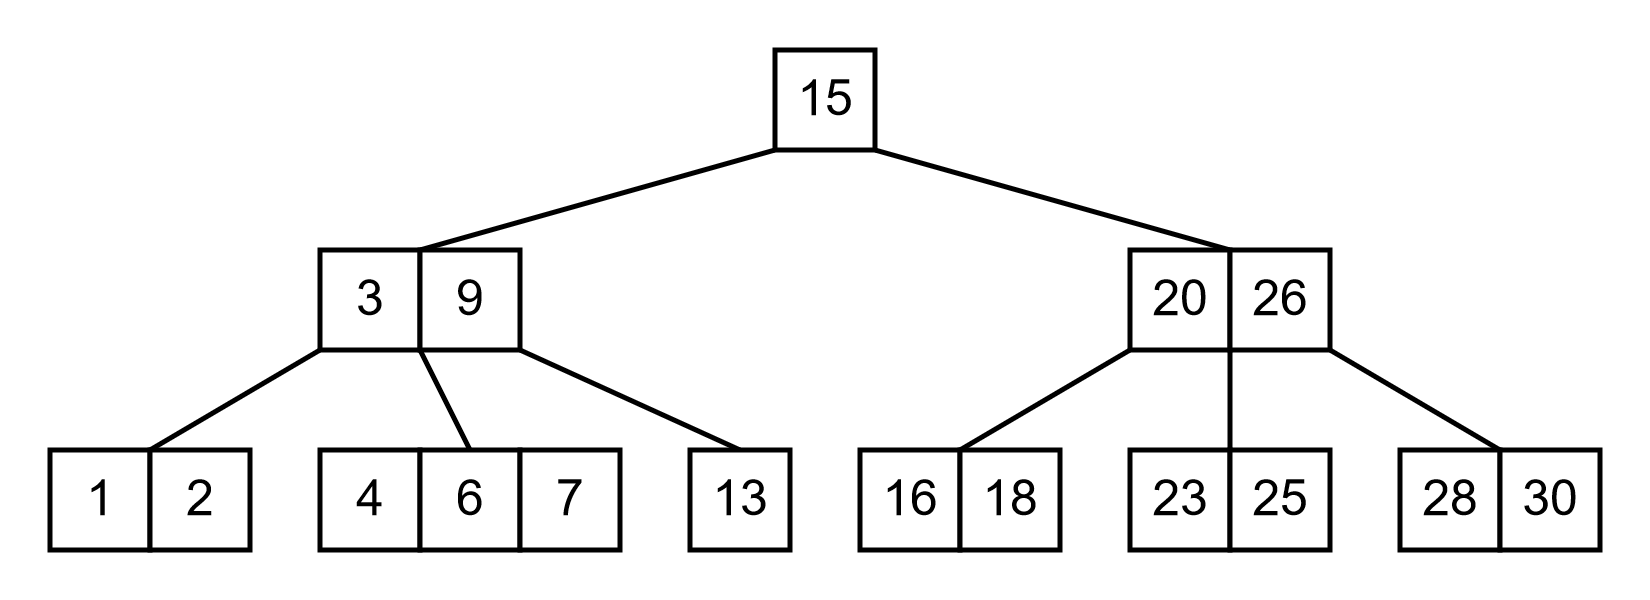
\includegraphics[width=\textwidth]{img/3c/8a}
            \end{subfigure}
            \begin{subfigure}[b]{0.45\textwidth}
                \centering
                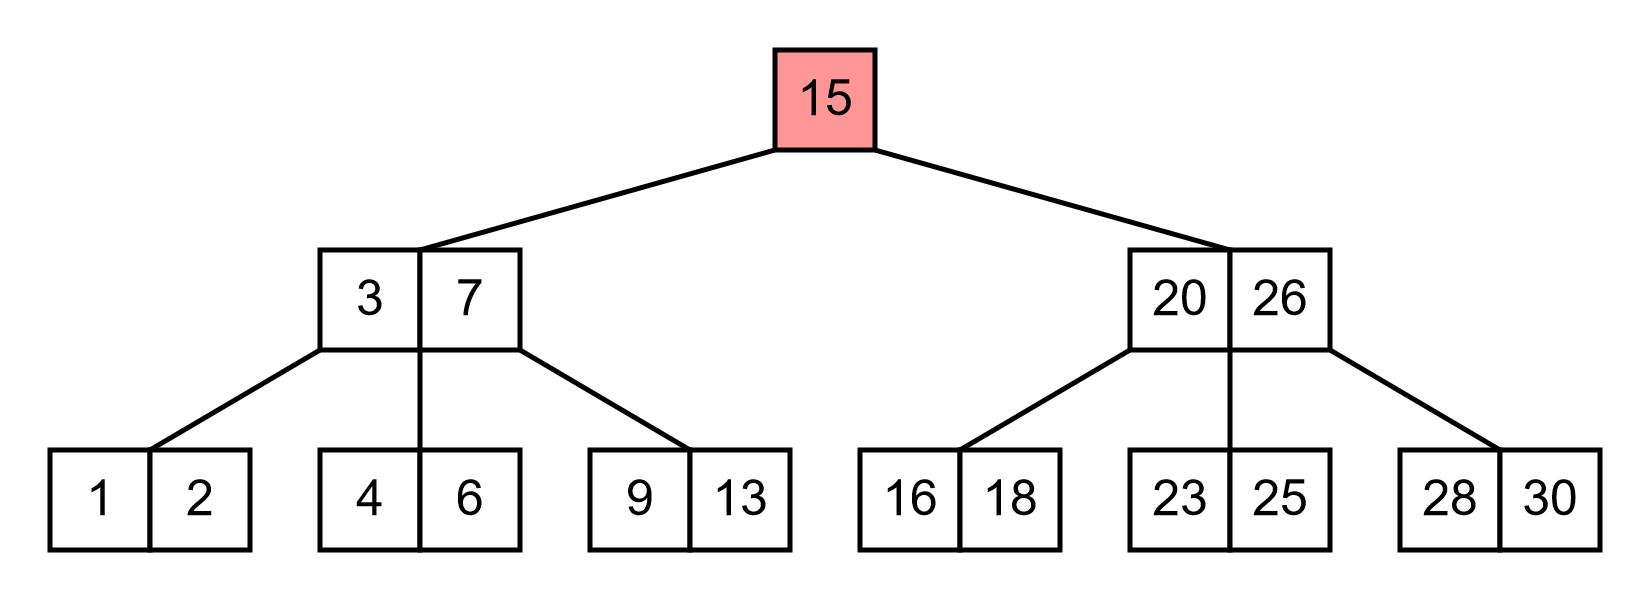
\includegraphics[width=\textwidth]{img/3c/9}
            \end{subfigure}
            \begin{subfigure}[b]{0.45\textwidth}
                \centering
                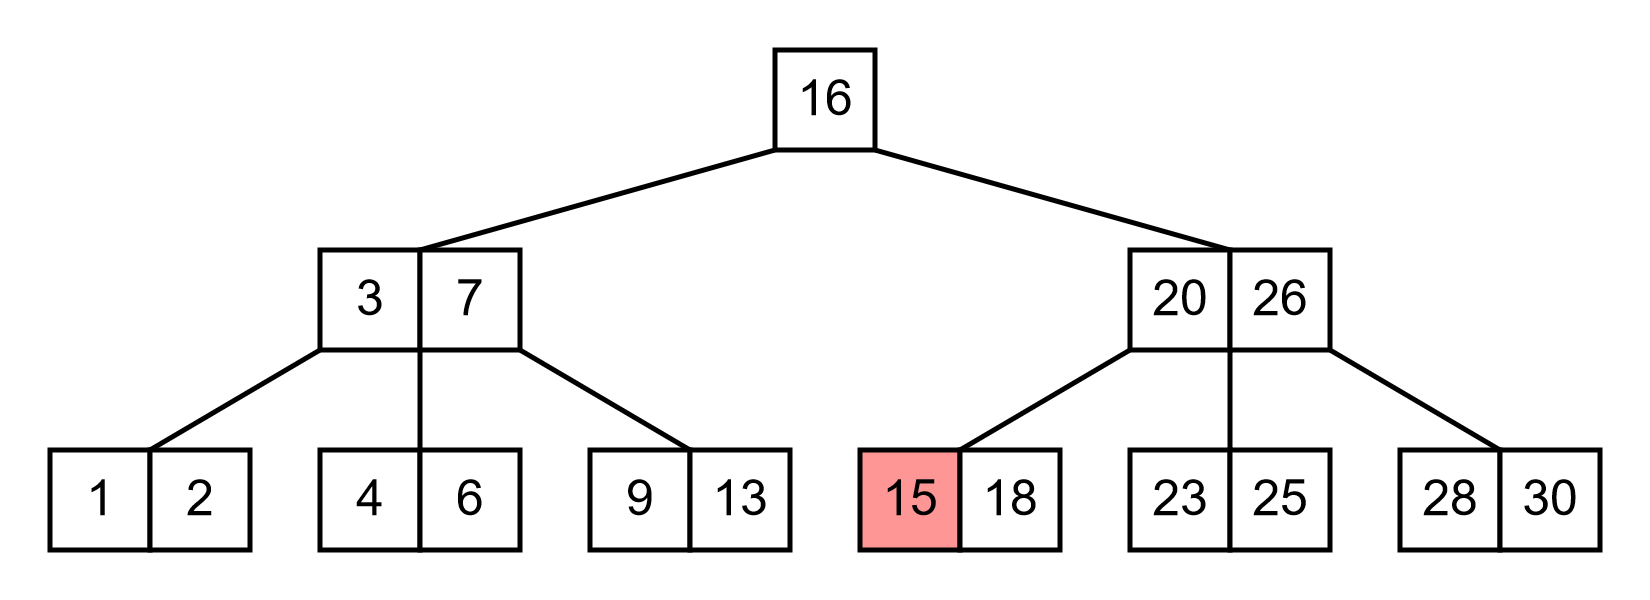
\includegraphics[width=\textwidth]{img/3c/10}
            \end{subfigure}
            \begin{subfigure}[b]{0.45\textwidth}
                \centering
                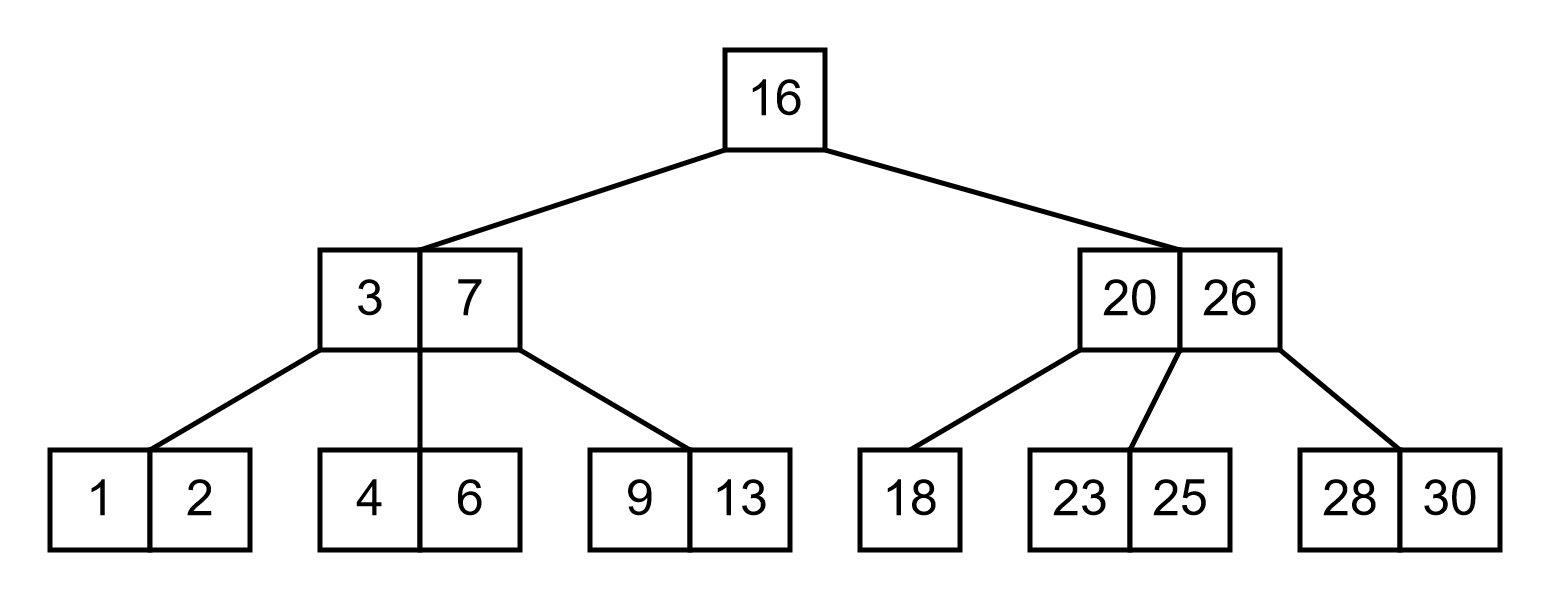
\includegraphics[width=\textwidth]{img/3c/11}
            \end{subfigure}
            \begin{subfigure}[b]{0.45\textwidth}
                \centering
                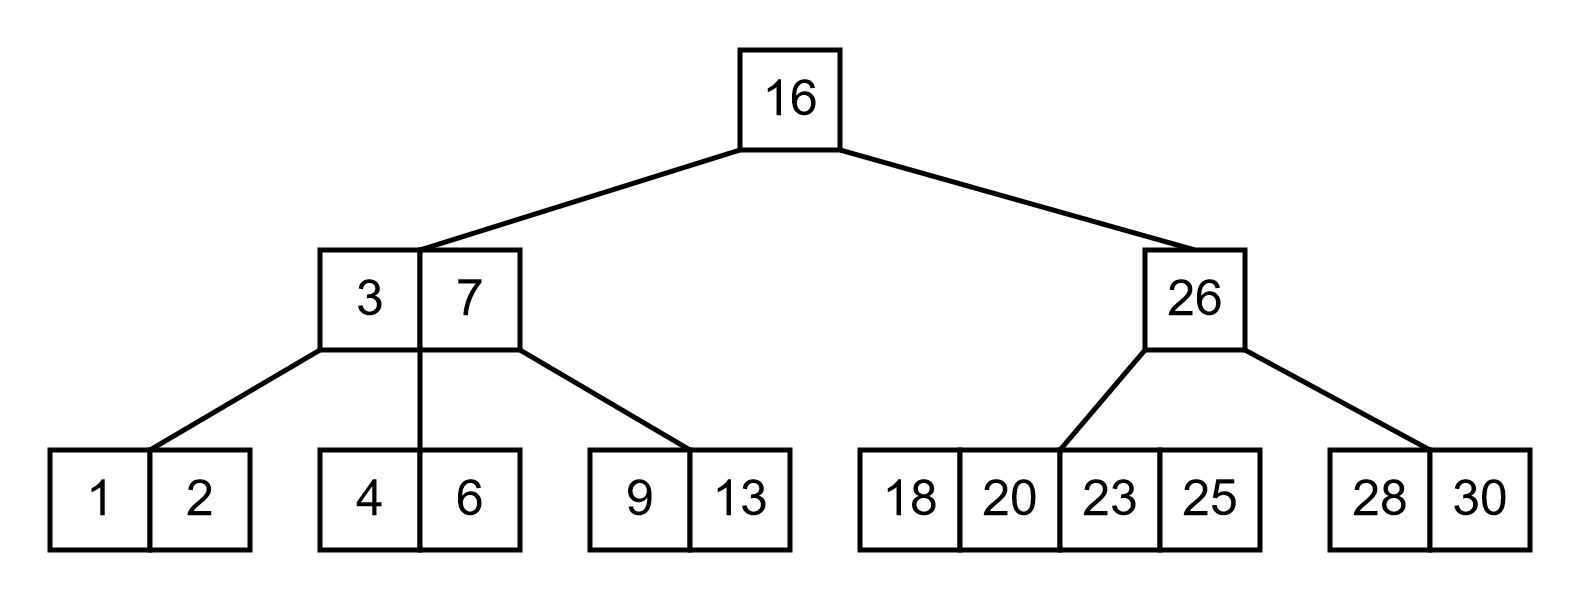
\includegraphics[width=\textwidth]{img/3c/12}
            \end{subfigure}
            \begin{subfigure}[b]{0.45\textwidth}
                \centering
                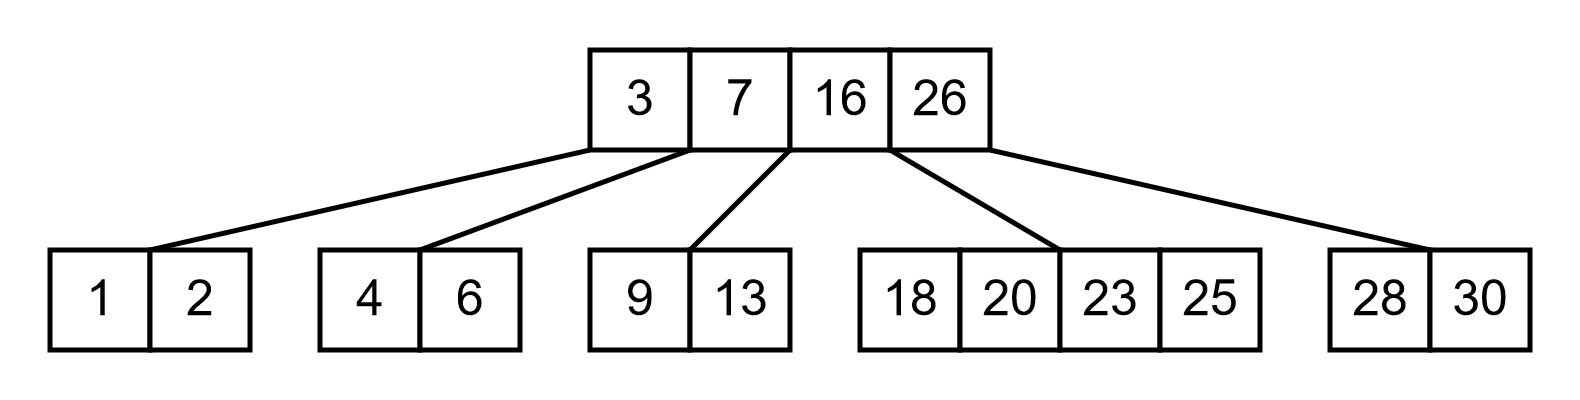
\includegraphics[width=\textwidth]{img/3c/13}
            \end{subfigure}
        \end{figure}
        \FloatBarrier

        \newpage
        \item \ \\
        \begin{figure}[h!]
            \centering
            \begin{subfigure}[b]{0.31\textwidth}
                \centering
                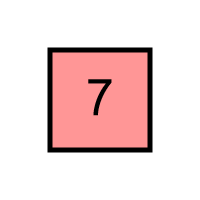
\includegraphics[scale=0.15]{img/3d/1}
            \end{subfigure}
            \begin{subfigure}[b]{0.31\textwidth}
                \centering
                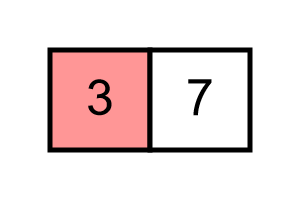
\includegraphics[scale=0.15]{img/3d/2}
            \end{subfigure}
            \begin{subfigure}[b]{0.31\textwidth}
                \centering
                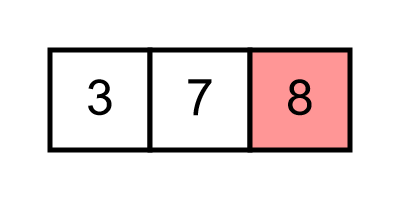
\includegraphics[scale=0.15]{img/3d/3}
            \end{subfigure}
            \begin{subfigure}[b]{0.31\textwidth}
                \centering
                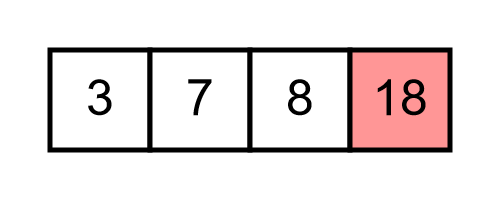
\includegraphics[scale=0.15]{img/3d/4}
            \end{subfigure}
            \begin{subfigure}[b]{0.31\textwidth}
                \centering
                \includegraphics[scale=0.15]{img/3d/5}
            \end{subfigure}
            \begin{subfigure}[b]{0.31\textwidth}
                \centering
                \includegraphics[scale=0.15]{img/3d/6}
            \end{subfigure}
            \begin{subfigure}[b]{0.31\textwidth}
                \centering
                \includegraphics[scale=0.15]{img/3d/7}
            \end{subfigure}
            \begin{subfigure}[b]{0.31\textwidth}
                \centering
                \includegraphics[scale=0.15]{img/3d/8}
            \end{subfigure}
            \begin{subfigure}[b]{0.31\textwidth}
                \centering
                \includegraphics[scale=0.15]{img/3d/9}
            \end{subfigure}
            \begin{subfigure}[b]{0.31\textwidth}
                \centering
                \includegraphics[scale=0.15]{img/3d/10}
            \end{subfigure}
            \begin{subfigure}[b]{0.31\textwidth}
                \centering
                \includegraphics[scale=0.15]{img/3d/11}
            \end{subfigure}
            \begin{subfigure}[b]{0.31\textwidth}
                \centering
                \includegraphics[scale=0.15]{img/3d/12}
            \end{subfigure}
            \begin{subfigure}[b]{0.31\textwidth}
                \centering
                \includegraphics[scale=0.14]{img/3d/13}
            \end{subfigure}
            \begin{subfigure}[b]{0.31\textwidth}
                \centering
                \includegraphics[scale=0.14]{img/3d/14}
            \end{subfigure}
            \begin{subfigure}[b]{0.31\textwidth}
                \centering
                \includegraphics[scale=0.14]{img/3d/15}
            \end{subfigure}
            \begin{subfigure}[b]{0.31\textwidth}
                \centering
                \includegraphics[scale=0.14]{img/3d/16}
            \end{subfigure}
        \end{figure}
        \FloatBarrier

        \newpage
        \item \ \\
        \begin{figure}[h!]
            \centering
            \begin{subfigure}[b]{0.31\textwidth}
                \centering
                \includegraphics[scale=0.15]{img/3e/2}
            \end{subfigure}
            \begin{subfigure}[b]{0.31\textwidth}
                \centering
                \includegraphics[scale=0.15]{img/3e/3}
            \end{subfigure}
            \begin{subfigure}[b]{0.31\textwidth}
                \centering
                \includegraphics[scale=0.15]{img/3e/4}
            \end{subfigure}
            \begin{subfigure}[b]{0.31\textwidth}
                \centering
                \includegraphics[scale=0.15]{img/3e/5}
            \end{subfigure}
            \begin{subfigure}[b]{0.31\textwidth}
                \centering
                \includegraphics[scale=0.15]{img/3e/6}
            \end{subfigure}
            \begin{subfigure}[b]{0.31\textwidth}
                \centering
                \includegraphics[scale=0.15]{img/3e/7}
            \end{subfigure}
            \begin{subfigure}[b]{0.31\textwidth}
                \centering
                \includegraphics[scale=0.15]{img/3e/8}
            \end{subfigure}
            \begin{subfigure}[b]{0.31\textwidth}
                \centering
                \includegraphics[scale=0.15]{img/3e/9}
            \end{subfigure}
            \begin{subfigure}[b]{0.31\textwidth}
                \centering
                \includegraphics[scale=0.15]{img/3e/10}
            \end{subfigure}
            \begin{subfigure}[b]{0.31\textwidth}
                \centering
                \includegraphics[scale=0.15]{img/3e/11}
            \end{subfigure}
            \begin{subfigure}[b]{0.31\textwidth}
                \centering
                \includegraphics[scale=0.15]{img/3e/12}
            \end{subfigure}
            \begin{subfigure}[b]{0.31\textwidth}
                \centering
                \includegraphics[scale=0.15]{img/3e/13}
            \end{subfigure}
            \begin{subfigure}[b]{0.31\textwidth}
                \centering
                \includegraphics[scale=0.15]{img/3e/14}
            \end{subfigure}
            \begin{subfigure}[b]{0.31\textwidth}
                \centering
                \includegraphics[scale=0.15]{img/3e/15}
            \end{subfigure}
            \begin{subfigure}[b]{0.31\textwidth}
                \centering
                \includegraphics[scale=0.15]{img/3e/16}
            \end{subfigure}
            \begin{subfigure}[b]{0.31\textwidth}
                \centering
                \includegraphics[scale=0.15]{img/3e/16a}
            \end{subfigure}
            \begin{subfigure}[b]{0.31\textwidth}
                \centering
                \includegraphics[scale=0.15]{img/3e/17}
            \end{subfigure}
            \begin{subfigure}[b]{0.31\textwidth}
                \centering
                \includegraphics[scale=0.15]{img/3e/18}
            \end{subfigure}
            \begin{subfigure}[b]{0.31\textwidth}
                \centering
                \includegraphics[scale=0.15]{img/3e/19}
            \end{subfigure}
        \end{figure}
        \FloatBarrier

        \newpage
        \item Bei der linearen Variante werden die Werte eines Knotens von links nach rechts durchlaufen.
        Sobald der gesuchte Wert kleiner ist, als der aktuelle Wert des Knotens, muss er sich (falls er überhaupt im Baum liegt) im entsprechenden Nachfolgerknoten befinden.
        Falls er größer ist als alle Werte des Knotens, muss es der letzte Nachfolger sein (Index: \texttt{nValues}).
        \begin{lstlisting}[language=c++]
bool searchLinear(Node *node, int value) {
    int i;
    for (i = 0; i < node->nValues; i++) {
        if (value < node->values[i]) break;
        if (value == node->values[i]) return true;
    }
    if (node->isLeaf) return false;
    return searchLinear(node->succ[i], value);
}
        \end{lstlisting}
        
        Für die zweite Variante wird der Wert in einem Knoten mittels binärer Suche gesucht.
        Was passiert, wenn der Wert nicht gefunden wird?
        Dieser Fall tritt immer dann ein, wenn während der Suche \texttt{start = end = middle} gilt und \texttt{values[middle]} nicht der gesuchte Wert ist.
        Falls \texttt{values[start]} zu groß ist, wird \texttt{end = middle + 1 = end + 1} gesetzt, andernfalls \texttt{start = middle - 1 = start - 1}.
        In beiden Fällen ist \texttt{start} anschließend der korrekte Nachfolgerindex.
        \begin{lstlisting}[language=c++]
bool searchBinary(Node *node, int value) {
    int start = 0;
    int end = node->nValues - 1;
    while (start <= end) {
        int middle = (start + end) / 2;
        if (value == node->values[middle]) return true;
        if (value < node->values[middle]) end = middle - 1;
        if (value > node->values[middle]) start = middle + 1;
    }
    if (node->isLeaf) return false;
    return searchLinear(node->succ[start], value);
}
        \end{lstlisting}

        \item Für beide Varianten ist die Worst-Case-Laufzeit gegeben durch die Anzahl der Knoten auf dem Pfad von der Wurzel zu einem Blatt, multipliziert mit dem Suchaufwand pro Knoten.
        Die maximale Anzahl der zu durchsuchenden Knoten ist $\log_{\lceil t / 2\lceil} \left(\frac{n - 1}{2}\right) + 1$ (siehe Vorlesung).
        \begin{align*}
            \log_{\lceil t / 2\lceil} \left(\frac{n - 1}{2}\right) + 1
            &= \log_{\lceil t / 2\lceil} (n - 1) - \log_{\lceil t / 2\lceil}(2) + 1 
            \leq \log_{\lceil t / 2\lceil} (n - 1) + 1  \\
            &= \frac{\log(n - 1)}{\log(\lceil t / 2\rceil)} + 1
            \leq \frac{\log(n - 1)}{\log(t / 2)} + 1
            = \frac{\log(n - 1)}{\log(t) - 1} + 1 \\
            &\leq \frac{\log(n - 1)}{\log(t) - \frac{1}{2}\log(t)} + 1
            = 2 \cdot \frac{\log(n - 1)}{\log(t)} + 1 = 2\log_t(n - 1) + 1 \\
            &\leq 2\log_t(n) + 1 \leq 2\log_t(n) + \log_t(n)
            &= O(\log_t(n))
        \end{align*}
        Der Worst-Case-Aufwand pro Knoten ist durch den Fall gegeben, dass der Knoten vollbesetzt ist, also $t - 1$ Elemente enthält.
        Bei der linearen Variante pro Knoten ist dieser Aufwand $O(t)$.
        Die Gesamtlaufzeit beträgt also $O(t \log_t(n))$.

        Der Aufwand pro Knoten bei Verwendung von binärer Suche beträgt im Worst Case $O(\log(t))$.
        Die Gesamtlaufzeit beträgt also $O(\log(t) \log_t(n))$.
        Da $\log_t(n) = \frac{\log(n)}{\log(t)}$, kann man $\log(t)$ kürzen und so die Laufzeit zu $O(\log(n))$ vereinfachen.
        Die Laufzeit bei Verwendung von binärer Suche ist also unabhängig von $t$.
    \end{enumerate}
\end{loesung}

\end{document}